%  LaTeX support: latex@mdpi.com
%  In case you need support, please attach all files that are necessary for compiling as well as the log file, and specify the details of your LaTeX setup (which operating system and LaTeX version / tools you are using).

%=================================================================
\documentclass[water,article,submit,moreauthors,pdftex]{mdpi}

% If you would like to post an early version of this manuscript as a preprint, you may use preprint as the journal and change 'submit' to 'accept'. The document class line would be, e.g., \documentclass[preprints,article,accept,moreauthors,pdftex]{mdpi}. This is especially recommended for submission to arXiv, where line numbers should be removed before posting. For preprints.org, the editorial staff will make this change immediately prior to posting.

%% Some pieces required from the pandoc template
\setlist[itemize]{leftmargin=*,labelsep=5.8mm}
\setlist[enumerate]{leftmargin=*,labelsep=4.9mm}


%--------------------
% Class Options:
%--------------------
%----------
% journal
%----------
% Choose between the following MDPI journals:
% acoustics, actuators, addictions, admsci, aerospace, agriculture, agriengineering, agronomy, algorithms, animals, antibiotics, antibodies, antioxidants, applsci, arts, asc, asi, atmosphere, atoms, axioms, batteries, bdcc, behavsci , beverages, bioengineering, biology, biomedicines, biomimetics, biomolecules, biosensors, brainsci , buildings, cancers, carbon , catalysts, cells, ceramics, challenges, chemengineering, chemistry, chemosensors, children, cleantechnol, climate, clockssleep, cmd, coatings, colloids, computation, computers, condensedmatter, cosmetics, cryptography, crystals, dairy, data, dentistry, designs , diagnostics, diseases, diversity, drones, econometrics, economies, education, electrochem, electronics, energies, entropy, environments, epigenomes, est, fermentation, fibers, fire, fishes, fluids, foods, forecasting, forests, fractalfract, futureinternet, futurephys, galaxies, games, gastrointestdisord, gels, genealogy, genes, geohazards, geosciences, geriatrics, hazardousmatters, healthcare, heritage, highthroughput, horticulturae, humanities, hydrology, ijerph, ijfs, ijgi, ijms, ijns, ijtpp, informatics, information, infrastructures, inorganics, insects, instruments, inventions, iot, j, jcdd, jcm, jcp, jcs, jdb, jfb, jfmk, jimaging, jintelligence, jlpea, jmmp, jmse, jnt, jof, joitmc, jpm, jrfm, jsan, land, languages, laws, life, literature, logistics, lubricants, machines, magnetochemistry, make, marinedrugs, materials, mathematics, mca, medicina, medicines, medsci, membranes, metabolites, metals, microarrays, micromachines, microorganisms, minerals, modelling, molbank, molecules, mps, mti, nanomaterials, ncrna, neuroglia, nitrogen, notspecified, nutrients, ohbm, particles, pathogens, pharmaceuticals, pharmaceutics, pharmacy, philosophies, photonics, physics, plants, plasma, polymers, polysaccharides, preprints , proceedings, processes, proteomes, psych, publications, quantumrep, quaternary, qubs, reactions, recycling, religions, remotesensing, reports, resources, risks, robotics, safety, sci, scipharm, sensors, separations, sexes, signals, sinusitis, smartcities, sna, societies, socsci, soilsystems, sports, standards, stats, surfaces, surgeries, sustainability, symmetry, systems, technologies, test, toxics, toxins, tropicalmed, universe, urbansci, vaccines, vehicles, vetsci, vibration, viruses, vision, water, wem, wevj

%---------
% article
%---------
% The default type of manuscript is "article", but can be replaced by:
% abstract, addendum, article, benchmark, book, bookreview, briefreport, casereport, changes, comment, commentary, communication, conceptpaper, conferenceproceedings, correction, conferencereport, expressionofconcern, extendedabstract, meetingreport, creative, datadescriptor, discussion, editorial, essay, erratum, hypothesis, interestingimages, letter, meetingreport, newbookreceived, obituary, opinion, projectreport, reply, retraction, review, perspective, protocol, shortnote, supfile, technicalnote, viewpoint
% supfile = supplementary materials

%----------
% submit
%----------
% The class option "submit" will be changed to "accept" by the Editorial Office when the paper is accepted. This will only make changes to the frontpage (e.g., the logo of the journal will get visible), the headings, and the copyright information. Also, line numbering will be removed. Journal info and pagination for accepted papers will also be assigned by the Editorial Office.

%------------------
% moreauthors
%------------------
% If there is only one author the class option oneauthor should be used. Otherwise use the class option moreauthors.

%---------
% pdftex
%---------
% The option pdftex is for use with pdfLaTeX. If eps figures are used, remove the option pdftex and use LaTeX and dvi2pdf.

%=================================================================
\firstpage{1}
\makeatletter
\setcounter{page}{\@firstpage}
\makeatother
\pubvolume{xx}
\issuenum{1}
\articlenumber{5}
\pubyear{2019}
\copyrightyear{2019}
%\externaleditor{Academic Editor: name}
\history{Received: date; Accepted: date; Published: date}
\updates{yes} % If there is an update available, un-comment this line

%% MDPI internal command: uncomment if new journal that already uses continuous page numbers
%\continuouspages{yes}

%------------------------------------------------------------------
% The following line should be uncommented if the LaTeX file is uploaded to arXiv.org
%\pdfoutput=1

%=================================================================
% Add packages and commands here. The following packages are loaded in our class file: fontenc, calc, indentfirst, fancyhdr, graphicx, lastpage, ifthen, lineno, float, amsmath, setspace, enumitem, mathpazo, booktabs, titlesec, etoolbox, amsthm, hyphenat, natbib, hyperref, footmisc, geometry, caption, url, mdframed, tabto, soul, multirow, microtype, tikz

%=================================================================
%% Please use the following mathematics environments: Theorem, Lemma, Corollary, Proposition, Characterization, Property, Problem, Example, ExamplesandDefinitions, Hypothesis, Remark, Definition
%% For proofs, please use the proof environment (the amsthm package is loaded by the MDPI class).

%=================================================================
% Full title of the paper (Capitalized)
\Title{Analysis of Access to Emergency Funds in Sub-Saharan Countries--
A Human Rights-Based Approach}

% Authors, for the paper (add full first names)
\Author{Rose
Porta$^{1,\ddagger,*}$\href{https://orcid.org/0000-0001-7296-6830}{\orcidicon}, Alejandra
Munoz
Garcia$^{1,\ddagger}$\href{https://orcid.org/0000-0002-9687-2342}{\orcidicon}, Margaret
Bassney$^{1,\ddagger}$\href{https://orcid.org/0000-0003-2843-6271}{\orcidicon}, Aushanae
Haller$^{1,\ddagger}$\href{https://orcid.org/0000-0002-2090-1952}{\orcidicon}}

% Authors, for metadata in PDF
\AuthorNames{Rose Porta, Alejandra Munoz Garcia, Margaret
Bassney, Aushanae Haller}

% Affiliations / Addresses (Add [1] after \address if there is only one affiliation.)
\address{%
$^{1}$ \quad Department of Statistical and Data Sciences, Smith College,
Northampton MA; \\
}
% Contact information of the corresponding author
\corres{Correspondence: \href{mailto:rporta@smith.edu}{\nolinkurl{rporta@smith.edu}}}

% Current address and/or shared authorship
\firstnote{These authors contributed equally to this work.}







% The commands \thirdnote{} till \eighthnote{} are available for further notes

% Simple summary
\simplesumm{A Simple summary goes here.}

% Abstract (Do not insert blank lines, i.e. \\)
\abstract{Having access to emergency funds is a valuable resource that
many people end up needing at least once in their lives. Those who have
access to emergency funding and other financial services have the
capacity to remain afloat when unexpected predicaments arise, while
those who are without this privilege have no choice but to endure crises
and simply hope for the best. The purpose of our project is to analyze
the access adults have to emergency funds and financial services in
Sub-Saharan countries using a 2017 dataset from the Global Findex
Database. Additionally, an important goal of our project is to employ a
variety of different approaches in an attempt to minimize bias and
maximize fairness, particularly when examining the performance for males
and females. We also aim to determine how adults in the Sub-Saharan
African region access financial services as well as establish the amount
of bias we have within our models using exploratory data analysis, a
baseline model, and a variety of fairness metrics. We hope to implement
our findings in a Jupyter notebook where this information can be made
accessible to a broader undergraduate audience.}

% Keywords
\keyword{keyword 1; keyword 2; keyword 3 (list three to ten pertinent
keywords specific to the article, yet reasonably common within the
subject discipline.).}

% The fields PACS, MSC, and JEL may be left empty or commented out if not applicable
%\PACS{J0101}
%\MSC{}
%\JEL{}

%%%%%%%%%%%%%%%%%%%%%%%%%%%%%%%%%%%%%%%%%%
% Only for the journal Diversity
%\LSID{\url{http://}}

%%%%%%%%%%%%%%%%%%%%%%%%%%%%%%%%%%%%%%%%%%
% Only for the journal Applied Sciences:
%\featuredapplication{Authors are encouraged to provide a concise description of the specific application or a potential application of the work. This section is not mandatory.}
%%%%%%%%%%%%%%%%%%%%%%%%%%%%%%%%%%%%%%%%%%

%%%%%%%%%%%%%%%%%%%%%%%%%%%%%%%%%%%%%%%%%%
% Only for the journal Data:
%\dataset{DOI number or link to the deposited data set in cases where the data set is published or set to be published separately. If the data set is submitted and will be published as a supplement to this paper in the journal Data, this field will be filled by the editors of the journal. In this case, please make sure to submit the data set as a supplement when entering your manuscript into our manuscript editorial system.}

%\datasetlicense{license under which the data set is made available (CC0, CC-BY, CC-BY-SA, CC-BY-NC, etc.)}

%%%%%%%%%%%%%%%%%%%%%%%%%%%%%%%%%%%%%%%%%%
% Only for the journal Toxins
%\keycontribution{The breakthroughs or highlights of the manuscript. Authors can write one or two sentences to describe the most important part of the paper.}

%\setcounter{secnumdepth}{4}
%%%%%%%%%%%%%%%%%%%%%%%%%%%%%%%%%%%%%%%%%%

% Pandoc syntax highlighting
\usepackage{color}
\usepackage{fancyvrb}
\newcommand{\VerbBar}{|}
\newcommand{\VERB}{\Verb[commandchars=\\\{\}]}
\DefineVerbatimEnvironment{Highlighting}{Verbatim}{commandchars=\\\{\}}
% Add ',fontsize=\small' for more characters per line
\usepackage{framed}
\definecolor{shadecolor}{RGB}{248,248,248}
\newenvironment{Shaded}{\begin{snugshade}}{\end{snugshade}}
\newcommand{\AlertTok}[1]{\textcolor[rgb]{0.94,0.16,0.16}{#1}}
\newcommand{\AnnotationTok}[1]{\textcolor[rgb]{0.56,0.35,0.01}{\textbf{\textit{#1}}}}
\newcommand{\AttributeTok}[1]{\textcolor[rgb]{0.77,0.63,0.00}{#1}}
\newcommand{\BaseNTok}[1]{\textcolor[rgb]{0.00,0.00,0.81}{#1}}
\newcommand{\BuiltInTok}[1]{#1}
\newcommand{\CharTok}[1]{\textcolor[rgb]{0.31,0.60,0.02}{#1}}
\newcommand{\CommentTok}[1]{\textcolor[rgb]{0.56,0.35,0.01}{\textit{#1}}}
\newcommand{\CommentVarTok}[1]{\textcolor[rgb]{0.56,0.35,0.01}{\textbf{\textit{#1}}}}
\newcommand{\ConstantTok}[1]{\textcolor[rgb]{0.00,0.00,0.00}{#1}}
\newcommand{\ControlFlowTok}[1]{\textcolor[rgb]{0.13,0.29,0.53}{\textbf{#1}}}
\newcommand{\DataTypeTok}[1]{\textcolor[rgb]{0.13,0.29,0.53}{#1}}
\newcommand{\DecValTok}[1]{\textcolor[rgb]{0.00,0.00,0.81}{#1}}
\newcommand{\DocumentationTok}[1]{\textcolor[rgb]{0.56,0.35,0.01}{\textbf{\textit{#1}}}}
\newcommand{\ErrorTok}[1]{\textcolor[rgb]{0.64,0.00,0.00}{\textbf{#1}}}
\newcommand{\ExtensionTok}[1]{#1}
\newcommand{\FloatTok}[1]{\textcolor[rgb]{0.00,0.00,0.81}{#1}}
\newcommand{\FunctionTok}[1]{\textcolor[rgb]{0.00,0.00,0.00}{#1}}
\newcommand{\ImportTok}[1]{#1}
\newcommand{\InformationTok}[1]{\textcolor[rgb]{0.56,0.35,0.01}{\textbf{\textit{#1}}}}
\newcommand{\KeywordTok}[1]{\textcolor[rgb]{0.13,0.29,0.53}{\textbf{#1}}}
\newcommand{\NormalTok}[1]{#1}
\newcommand{\OperatorTok}[1]{\textcolor[rgb]{0.81,0.36,0.00}{\textbf{#1}}}
\newcommand{\OtherTok}[1]{\textcolor[rgb]{0.56,0.35,0.01}{#1}}
\newcommand{\PreprocessorTok}[1]{\textcolor[rgb]{0.56,0.35,0.01}{\textit{#1}}}
\newcommand{\RegionMarkerTok}[1]{#1}
\newcommand{\SpecialCharTok}[1]{\textcolor[rgb]{0.00,0.00,0.00}{#1}}
\newcommand{\SpecialStringTok}[1]{\textcolor[rgb]{0.31,0.60,0.02}{#1}}
\newcommand{\StringTok}[1]{\textcolor[rgb]{0.31,0.60,0.02}{#1}}
\newcommand{\VariableTok}[1]{\textcolor[rgb]{0.00,0.00,0.00}{#1}}
\newcommand{\VerbatimStringTok}[1]{\textcolor[rgb]{0.31,0.60,0.02}{#1}}
\newcommand{\WarningTok}[1]{\textcolor[rgb]{0.56,0.35,0.01}{\textbf{\textit{#1}}}}

% tightlist command for lists without linebreak
\providecommand{\tightlist}{%
  \setlength{\itemsep}{0pt}\setlength{\parskip}{0pt}}




\begin{document}


%%%%%%%%%%%%%%%%%%%%%%%%%%%%%%%%%%%%%%%%%%

\begin{Shaded}
\begin{Highlighting}[]
\CommentTok{\# !pip install seaborn}
\CommentTok{\# !pip install numpy}
\CommentTok{\# !pip install pandas}
\CommentTok{\# !pip install matplotlib}
\end{Highlighting}
\end{Shaded}

\begin{Shaded}
\begin{Highlighting}[]
\CommentTok{\# test python chunk}

\CommentTok{\# Imports}
\ImportTok{import}\NormalTok{ pandas }\ImportTok{as}\NormalTok{ pd}
\ImportTok{import}\NormalTok{ numpy }\ImportTok{as}\NormalTok{ np}
\ImportTok{import}\NormalTok{ seaborn }\ImportTok{as}\NormalTok{ sns}
\CommentTok{\# from plotnine import *}
\ImportTok{import}\NormalTok{ matplotlib.pyplot }\ImportTok{as}\NormalTok{ plt}
\CommentTok{\# from sklearn.model\_selection import train\_test\_split}
\CommentTok{\# from sklearn.tree import DecisionTreeRegressor}
\CommentTok{\# import statsmodels.api as sm}
\CommentTok{\# from sklearn.compose import make\_column\_transformer}
\CommentTok{\# from sklearn.preprocessing import OneHotEncoder}
\CommentTok{\# from sklearn.linear\_model import LogisticRegression, LogisticRegressionCV}
\end{Highlighting}
\end{Shaded}

\hypertarget{version}{%
\section{Version}\label{version}}

This Rmd-skeleton uses the mdpi Latex template published 2019/02.
However, the official template gets more frequently updated than the
`rticles' package. Therefore, please make sure prior to paper
submission, that you're using the most recent .cls, .tex and .bst files
(available \href{http://www.mdpi.com/authors/latex}{here}).

\hypertarget{introduction}{%
\section{Introduction}\label{introduction}}

Science is often viewed as a way to offer trustworthy research backed
solutions and answers. A lot of that research involves statistical
methods performed on data however, what happens when the data and
statistical methods are not as objective and trustworthy as is so often
assumed? The conclusions drawn from the data are biased and unfair, most
often towards minorities and protected classes of people. To contribute
to a human rights based approach to data analysis, we evaluate fairness
metrics on a machine learning algorithm to measure bias. We use a Global
Findex data set which contains financial information about 35 Sub
Saharan countries. Specifically, we create models to predict access to
emergency funds, then analyze the fairness of those models. We focus on
group and individual fairness metrics for the protected attribute sex.
In addition we investigate the data set itself to understand where
potential biases might have been implanted.

Data sets and algorithms have real world impacts on real people. The
inherent bias in data sets can carry over into machine learning
algorithms that are used to profile and categorize people
\citep{navarro2021risk, hellstrom2020bias}. Since data set's are not
collected in a vacuum and often represent the discriminatory
environments in which they are collected
\citep{barocas_fairness_nodate}, we must find ways to make data sets and
statistical methods more equitable. In this study we explore fairness
methods that can be used to evaluate machine learning models. The
``impossibility theorem'' is the idea that not all fairness metrics can
be satisfied at the same time\citep{kleinberg2016inherent}. Although
fairness is complex and there are multiple approaches to make a model
fair \citep{kypraiou_what_2021, green2018myth}, it's important to
continue to question how data and algorithms can be biased and how to
mitigate that bias.

While there have been previous studies implementing fairness techniques
in different contexts\citep{deho2022existing, kim2022information}, we
implement them in an exploratory context meant to teach how and when to
use these techniques thus giving us more freedom to branch beyond a
specific question while supporting previous work about the importance of
these fairness metrics\citep{anahideh2022fair, barocas_fairness_nodate}.
We analyse the data, data collection methods, prediction models, and the
fairness metrics to assess how biased our data is and understand how we
can de-bias when possible.

\hypertarget{data}{%
\section{Data}\label{data}}

Our data is derived from The World Bank in The Global Findex Database,
comprising the most comprehensive data sets on how adults save, borrow,
make payments, and manage risk in more than 140 economies around the
world. The data set was created to record various measures of financial
equity and inclusion, with the intention that such information could
reveal opportunities to expand access to financial services and to
promote greater use of digital financial services for individuals who do
not have a bank account. Conducted by Gallup, Inc for the annual Gallup
World Poll, the participants responded to the questionnaire either on
the phone or in-person. There were several variables of interest in this
dataset when creating models to predict access to emergency funds,
including demographic and financial information.

\begin{Shaded}
\begin{Highlighting}[]
\CommentTok{\# Read in Data}
\BuiltInTok{file} \OperatorTok{=} \StringTok{\textquotesingle{}\textasciitilde{}/Desktop/Fall{-}2022/SDS410/women{-}at{-}table/findex\_SubSahAfrica.csv\textquotesingle{}}
\NormalTok{df }\OperatorTok{=}\NormalTok{ pd.read\_csv(}\BuiltInTok{file}\NormalTok{, index\_col}\OperatorTok{=}\DecValTok{0}\NormalTok{)}
\BuiltInTok{print}\NormalTok{(}\SpecialStringTok{f\textquotesingle{}There are }\SpecialCharTok{\{}\NormalTok{df}\SpecialCharTok{.}\NormalTok{shape[}\DecValTok{0}\NormalTok{]}\SpecialCharTok{\}}\SpecialStringTok{ entries and }\SpecialCharTok{\{}\NormalTok{df}\SpecialCharTok{.}\NormalTok{shape[}\DecValTok{1}\NormalTok{]}\SpecialCharTok{\}}\SpecialStringTok{ features\textquotesingle{}}\NormalTok{)}
\end{Highlighting}
\end{Shaded}

\begin{verbatim}
## There are 35000 entries and 105 features
\end{verbatim}

\begin{Shaded}
\begin{Highlighting}[]
\NormalTok{df.head()}
\end{Highlighting}
\end{Shaded}

\begin{verbatim}
##       economy economycode  ... pay_cash  pay_cash_mobintbuy
## 12138   Benin         BEN  ...      0.0                 NaN
## 12139   Benin         BEN  ...      0.0                 NaN
## 12140   Benin         BEN  ...      0.0                 0.0
## 12141   Benin         BEN  ...      0.0                 NaN
## 12142   Benin         BEN  ...      0.0                 NaN
## 
## [5 rows x 105 columns]
\end{verbatim}

\begin{Shaded}
\begin{Highlighting}[]
\CommentTok{\# Set Gender Palette}
\NormalTok{red }\OperatorTok{=} \StringTok{\textquotesingle{}\#FF7377\textquotesingle{}}
\NormalTok{blue }\OperatorTok{=} \StringTok{\textquotesingle{}\#00B2EE\textquotesingle{}}
\NormalTok{gender\_palette }\OperatorTok{=}\NormalTok{ [blue, red]}

\NormalTok{purple }\OperatorTok{=} \StringTok{\textquotesingle{}\#BF3EFF\textquotesingle{}}
\NormalTok{green }\OperatorTok{=} \StringTok{\textquotesingle{}\#1B851B\textquotesingle{}}
\NormalTok{yes\_no\_pal }\OperatorTok{=}\NormalTok{ [purple, green]}

\NormalTok{pink }\OperatorTok{=} \StringTok{\textquotesingle{}\#FFC0CB\textquotesingle{}}
\end{Highlighting}
\end{Shaded}

\begin{Shaded}
\begin{Highlighting}[]
\CommentTok{\# select vars of interest}
\NormalTok{df2 }\OperatorTok{=}\NormalTok{ df[[}\StringTok{\textquotesingle{}female\textquotesingle{}}\NormalTok{, }\StringTok{\textquotesingle{}age\textquotesingle{}}\NormalTok{, }\StringTok{\textquotesingle{}emp\_in\textquotesingle{}}\NormalTok{, }\StringTok{\textquotesingle{}account\_fin\textquotesingle{}}\NormalTok{, }\StringTok{\textquotesingle{}fin24\textquotesingle{}}\NormalTok{, }\StringTok{\textquotesingle{}fin25\textquotesingle{}}\NormalTok{, }\StringTok{\textquotesingle{}fin32\textquotesingle{}}\NormalTok{, }\StringTok{\textquotesingle{}fin48\textquotesingle{}}\NormalTok{, }\StringTok{\textquotesingle{}educ\textquotesingle{}}\NormalTok{, }\StringTok{\textquotesingle{}economy\textquotesingle{}}\NormalTok{]]}
\NormalTok{df2 }\OperatorTok{=}\NormalTok{ df2.query(}\StringTok{\textquotesingle{}fin24 \textless{} 3\textquotesingle{}}\NormalTok{)}
\CommentTok{\# Recode fin24 values}
\NormalTok{df2.loc[df2[}\StringTok{\textquotesingle{}fin24\textquotesingle{}}\NormalTok{] }\OperatorTok{==} \DecValTok{1}\NormalTok{, }\StringTok{"fin24"}\NormalTok{] }\OperatorTok{=} \StringTok{\textquotesingle{}Yes\textquotesingle{}}
\NormalTok{df2.loc[df2[}\StringTok{\textquotesingle{}fin24\textquotesingle{}}\NormalTok{] }\OperatorTok{==} \DecValTok{2}\NormalTok{, }\StringTok{"fin24"}\NormalTok{] }\OperatorTok{=} \StringTok{\textquotesingle{}No\textquotesingle{}}
\NormalTok{df2.loc[df2[}\StringTok{\textquotesingle{}fin24\textquotesingle{}}\NormalTok{] }\OperatorTok{==} \DecValTok{3}\NormalTok{, }\StringTok{"fin24"}\NormalTok{] }\OperatorTok{=} \StringTok{\textquotesingle{}Don}\CharTok{\textbackslash{}\textquotesingle{}}\StringTok{t Know\textquotesingle{}}
\NormalTok{df2.loc[df2[}\StringTok{\textquotesingle{}fin24\textquotesingle{}}\NormalTok{] }\OperatorTok{==} \DecValTok{4}\NormalTok{, }\StringTok{"fin24"}\NormalTok{] }\OperatorTok{=} \StringTok{\textquotesingle{}Refuse\textquotesingle{}}
\CommentTok{\# rename fin24 to has\_access}
\NormalTok{df2.rename(columns }\OperatorTok{=}\NormalTok{ \{}\StringTok{\textquotesingle{}fin24\textquotesingle{}}\NormalTok{: }\StringTok{\textquotesingle{}has\_access\textquotesingle{}}\NormalTok{\}, inplace }\OperatorTok{=} \VariableTok{True}\NormalTok{)}
\CommentTok{\# recode gender}
\NormalTok{df2.loc[df2[}\StringTok{\textquotesingle{}female\textquotesingle{}}\NormalTok{] }\OperatorTok{==} \DecValTok{1}\NormalTok{, }\StringTok{"female"}\NormalTok{] }\OperatorTok{=} \StringTok{\textquotesingle{}male\textquotesingle{}}
\NormalTok{df2.loc[df2[}\StringTok{\textquotesingle{}female\textquotesingle{}}\NormalTok{] }\OperatorTok{==} \DecValTok{2}\NormalTok{, }\StringTok{"female"}\NormalTok{] }\OperatorTok{=} \StringTok{\textquotesingle{}female\textquotesingle{}}
\NormalTok{df2.rename(columns }\OperatorTok{=}\NormalTok{ \{}\StringTok{\textquotesingle{}female\textquotesingle{}}\NormalTok{: }\StringTok{\textquotesingle{}gender\textquotesingle{}}\NormalTok{\}, inplace }\OperatorTok{=} \VariableTok{True}\NormalTok{)}
\CommentTok{\# recode account\_fin}
\NormalTok{df2.loc[df2[}\StringTok{\textquotesingle{}account\_fin\textquotesingle{}}\NormalTok{] }\OperatorTok{==} \DecValTok{0}\NormalTok{, }\StringTok{"account\_fin"}\NormalTok{] }\OperatorTok{=} \StringTok{\textquotesingle{}No\textquotesingle{}}
\NormalTok{df2.loc[df2[}\StringTok{\textquotesingle{}account\_fin\textquotesingle{}}\NormalTok{] }\OperatorTok{==} \DecValTok{1}\NormalTok{, }\StringTok{"account\_fin"}\NormalTok{] }\OperatorTok{=} \StringTok{\textquotesingle{}Yes\textquotesingle{}}
\CommentTok{\# recode emp\_in}
\NormalTok{df2.loc[df2[}\StringTok{\textquotesingle{}emp\_in\textquotesingle{}}\NormalTok{] }\OperatorTok{==} \DecValTok{0}\NormalTok{, }\StringTok{"emp\_in"}\NormalTok{] }\OperatorTok{=} \StringTok{\textquotesingle{}No\textquotesingle{}}
\NormalTok{df2.loc[df2[}\StringTok{\textquotesingle{}emp\_in\textquotesingle{}}\NormalTok{] }\OperatorTok{==} \DecValTok{1}\NormalTok{, }\StringTok{"emp\_in"}\NormalTok{] }\OperatorTok{=} \StringTok{\textquotesingle{}Yes\textquotesingle{}}
\CommentTok{\# Recode fin32 values: Recieved Wage Payments}
\NormalTok{df2.loc[df2[}\StringTok{\textquotesingle{}fin32\textquotesingle{}}\NormalTok{] }\OperatorTok{==} \DecValTok{1}\NormalTok{, }\StringTok{"fin32"}\NormalTok{] }\OperatorTok{=} \StringTok{\textquotesingle{}Yes\textquotesingle{}}
\NormalTok{df2.loc[df2[}\StringTok{\textquotesingle{}fin32\textquotesingle{}}\NormalTok{] }\OperatorTok{==} \DecValTok{2}\NormalTok{, }\StringTok{"fin32"}\NormalTok{] }\OperatorTok{=} \StringTok{\textquotesingle{}No\textquotesingle{}}
\NormalTok{df2.loc[df2[}\StringTok{\textquotesingle{}fin32\textquotesingle{}}\NormalTok{] }\OperatorTok{==} \DecValTok{3}\NormalTok{, }\StringTok{"fin32"}\NormalTok{] }\OperatorTok{=} \StringTok{\textquotesingle{}Don}\CharTok{\textbackslash{}\textquotesingle{}}\StringTok{t Know\textquotesingle{}}
\NormalTok{df2.loc[df2[}\StringTok{\textquotesingle{}fin32\textquotesingle{}}\NormalTok{] }\OperatorTok{==} \DecValTok{4}\NormalTok{, }\StringTok{"fin32"}\NormalTok{] }\OperatorTok{=} \StringTok{\textquotesingle{}Refuse\textquotesingle{}}
\CommentTok{\# recode fin48 values: National ID}
\NormalTok{df2.loc[df2[}\StringTok{\textquotesingle{}fin48\textquotesingle{}}\NormalTok{] }\OperatorTok{==} \DecValTok{1}\NormalTok{, }\StringTok{"fin48"}\NormalTok{] }\OperatorTok{=} \StringTok{\textquotesingle{}Yes\textquotesingle{}}
\NormalTok{df2.loc[df2[}\StringTok{\textquotesingle{}fin48\textquotesingle{}}\NormalTok{] }\OperatorTok{==} \DecValTok{2}\NormalTok{, }\StringTok{"fin48"}\NormalTok{] }\OperatorTok{=} \StringTok{\textquotesingle{}No\textquotesingle{}}
\NormalTok{df2.loc[df2[}\StringTok{\textquotesingle{}fin48\textquotesingle{}}\NormalTok{] }\OperatorTok{==} \DecValTok{3}\NormalTok{, }\StringTok{"fin48"}\NormalTok{] }\OperatorTok{=} \StringTok{\textquotesingle{}Don}\CharTok{\textbackslash{}\textquotesingle{}}\StringTok{t Know\textquotesingle{}}
\NormalTok{df2.loc[df2[}\StringTok{\textquotesingle{}fin48\textquotesingle{}}\NormalTok{] }\OperatorTok{==} \DecValTok{4}\NormalTok{, }\StringTok{"fin48"}\NormalTok{] }\OperatorTok{=} \StringTok{\textquotesingle{}Refuse\textquotesingle{}}
\CommentTok{\#recode educ values: Highest Level of Education}
\NormalTok{df2.loc[df2[}\StringTok{\textquotesingle{}educ\textquotesingle{}}\NormalTok{] }\OperatorTok{==} \DecValTok{1}\NormalTok{, }\StringTok{"educ"}\NormalTok{] }\OperatorTok{=} \StringTok{\textquotesingle{}Primary\textquotesingle{}}
\NormalTok{df2.loc[df2[}\StringTok{\textquotesingle{}educ\textquotesingle{}}\NormalTok{] }\OperatorTok{==} \DecValTok{2}\NormalTok{, }\StringTok{"educ"}\NormalTok{] }\OperatorTok{=} \StringTok{\textquotesingle{}Secondary\textquotesingle{}}
\NormalTok{df2.loc[df2[}\StringTok{\textquotesingle{}educ\textquotesingle{}}\NormalTok{] }\OperatorTok{==} \DecValTok{3}\NormalTok{, }\StringTok{"educ"}\NormalTok{] }\OperatorTok{=} \StringTok{\textquotesingle{}Tertiary\textquotesingle{}}
\NormalTok{df2.loc[df2[}\StringTok{\textquotesingle{}educ\textquotesingle{}}\NormalTok{] }\OperatorTok{==} \DecValTok{4}\NormalTok{, }\StringTok{"educ"}\NormalTok{] }\OperatorTok{=} \StringTok{\textquotesingle{}Don}\CharTok{\textbackslash{}\textquotesingle{}}\StringTok{t Know\textquotesingle{}}
\NormalTok{df2.loc[df2[}\StringTok{\textquotesingle{}educ\textquotesingle{}}\NormalTok{] }\OperatorTok{==} \DecValTok{5}\NormalTok{, }\StringTok{"educ"}\NormalTok{] }\OperatorTok{=} \StringTok{\textquotesingle{}Refuse\textquotesingle{}}
\CommentTok{\#recode fin25 values: Main Source of Emergency Funds}
\NormalTok{df2.loc[df2[}\StringTok{\textquotesingle{}fin25\textquotesingle{}}\NormalTok{] }\OperatorTok{==} \DecValTok{1}\NormalTok{, }\StringTok{"fin25"}\NormalTok{] }\OperatorTok{=} \StringTok{\textquotesingle{}Savings\textquotesingle{}}
\NormalTok{df2.loc[df2[}\StringTok{\textquotesingle{}fin25\textquotesingle{}}\NormalTok{] }\OperatorTok{==} \DecValTok{2}\NormalTok{, }\StringTok{"fin25"}\NormalTok{] }\OperatorTok{=} \StringTok{\textquotesingle{}Family, relatives, or friends\textquotesingle{}}
\NormalTok{df2.loc[df2[}\StringTok{\textquotesingle{}fin25\textquotesingle{}}\NormalTok{] }\OperatorTok{==} \DecValTok{3}\NormalTok{, }\StringTok{"fin25"}\NormalTok{] }\OperatorTok{=} \StringTok{\textquotesingle{}Money from working\textquotesingle{}}
\NormalTok{df2.loc[df2[}\StringTok{\textquotesingle{}fin25\textquotesingle{}}\NormalTok{] }\OperatorTok{==} \DecValTok{4}\NormalTok{, }\StringTok{"fin25"}\NormalTok{] }\OperatorTok{=} \StringTok{\textquotesingle{}Borrowing from a bank/employer/private lender\textquotesingle{}}
\NormalTok{df2.loc[df2[}\StringTok{\textquotesingle{}fin25\textquotesingle{}}\NormalTok{] }\OperatorTok{==} \DecValTok{5}\NormalTok{, }\StringTok{"fin25"}\NormalTok{] }\OperatorTok{=} \StringTok{\textquotesingle{}Selling assets\textquotesingle{}}
\NormalTok{df2.loc[df2[}\StringTok{\textquotesingle{}fin25\textquotesingle{}}\NormalTok{] }\OperatorTok{==} \DecValTok{6}\NormalTok{, }\StringTok{"fin25"}\NormalTok{] }\OperatorTok{=} \StringTok{\textquotesingle{}(Some other source)\textquotesingle{}}
\NormalTok{df2.loc[df2[}\StringTok{\textquotesingle{}fin25\textquotesingle{}}\NormalTok{] }\OperatorTok{==} \DecValTok{7}\NormalTok{, }\StringTok{"fin25"}\NormalTok{] }\OperatorTok{=} \StringTok{\textquotesingle{}Don}\CharTok{\textbackslash{}\textquotesingle{}}\StringTok{t Know\textquotesingle{}}
\NormalTok{df2.loc[df2[}\StringTok{\textquotesingle{}fin25\textquotesingle{}}\NormalTok{] }\OperatorTok{==} \DecValTok{8}\NormalTok{, }\StringTok{"fin25"}\NormalTok{] }\OperatorTok{=} \StringTok{\textquotesingle{}Refuse\textquotesingle{}}
\CommentTok{\#recode fin32 values: Recieved Wage Payments}
\NormalTok{df2.loc[df2[}\StringTok{\textquotesingle{}fin32\textquotesingle{}}\NormalTok{] }\OperatorTok{==} \DecValTok{1}\NormalTok{, }\StringTok{"fin32"}\NormalTok{] }\OperatorTok{=} \StringTok{\textquotesingle{}Yes\textquotesingle{}}
\NormalTok{df2.loc[df2[}\StringTok{\textquotesingle{}fin32\textquotesingle{}}\NormalTok{] }\OperatorTok{==} \DecValTok{2}\NormalTok{, }\StringTok{"fin32"}\NormalTok{] }\OperatorTok{=} \StringTok{\textquotesingle{}No\textquotesingle{}}
\NormalTok{df2.loc[df2[}\StringTok{\textquotesingle{}fin32\textquotesingle{}}\NormalTok{] }\OperatorTok{==} \DecValTok{3}\NormalTok{, }\StringTok{"fin32"}\NormalTok{] }\OperatorTok{=} \StringTok{\textquotesingle{}Don}\CharTok{\textbackslash{}\textquotesingle{}}\StringTok{t Know\textquotesingle{}}
\NormalTok{df2.loc[df2[}\StringTok{\textquotesingle{}fin32\textquotesingle{}}\NormalTok{] }\OperatorTok{==} \DecValTok{4}\NormalTok{, }\StringTok{"fin32"}\NormalTok{] }\OperatorTok{=} \StringTok{\textquotesingle{}Refuse\textquotesingle{}}

\NormalTok{df2.rename(columns }\OperatorTok{=}\NormalTok{ \{}\StringTok{\textquotesingle{}fin32\textquotesingle{}}\NormalTok{: }\StringTok{\textquotesingle{}Receive Wage Payments\textquotesingle{}}\NormalTok{, }\StringTok{\textquotesingle{}fin48\textquotesingle{}}\NormalTok{: }\StringTok{\textquotesingle{}National ID\textquotesingle{}}\NormalTok{, }\StringTok{\textquotesingle{}educ\textquotesingle{}}\NormalTok{: }\StringTok{\textquotesingle{}Education\textquotesingle{}}\NormalTok{, }\StringTok{\textquotesingle{}fin25\textquotesingle{}}\NormalTok{: }\StringTok{\textquotesingle{}main\_source\_funds\textquotesingle{}}\NormalTok{\}, inplace }\OperatorTok{=} \VariableTok{True}\NormalTok{)}
\NormalTok{df2.head()}
\end{Highlighting}
\end{Shaded}

\begin{verbatim}
##        gender   age emp_in  ... National ID Education economy
## 12138    male  60.0     No  ...          No   Primary   Benin
## 12139    male  45.0    Yes  ...         Yes   Primary   Benin
## 12140    male  27.0    Yes  ...         Yes  Tertiary   Benin
## 12141  female  24.0    Yes  ...          No   Primary   Benin
## 12142    male  22.0    Yes  ...          No   Primary   Benin
## 
## [5 rows x 10 columns]
\end{verbatim}

\hypertarget{demographics}{%
\subsection{Demographics}\label{demographics}}

\hypertarget{gender}{%
\subsubsection{\texorpdfstring{\emph{gender}}{gender}}\label{gender}}

The variable \emph{gender} distinguishes gender. There are 16,716 males
in this dataset and 17,388 females. This is a fairly equal distribution
that we can see in the graph below.

\begin{Shaded}
\begin{Highlighting}[]
\CommentTok{\# barplot female versus not}
\NormalTok{g }\OperatorTok{=}\NormalTok{ sns.countplot(x }\OperatorTok{=} \StringTok{\textquotesingle{}gender\textquotesingle{}}\NormalTok{, data }\OperatorTok{=}\NormalTok{ df2, palette }\OperatorTok{=}\NormalTok{ gender\_palette)}
\ControlFlowTok{for}\NormalTok{ p }\KeywordTok{in}\NormalTok{ g.patches:}
\NormalTok{   g.annotate(}\StringTok{\textquotesingle{}}\SpecialCharTok{\{:.1f\}}\StringTok{\textquotesingle{}}\NormalTok{.}\BuiltInTok{format}\NormalTok{(p.get\_height()), (p.get\_x()}\OperatorTok{+} \FloatTok{.3}\NormalTok{, p.get\_height()}\OperatorTok{+}\DecValTok{100}\NormalTok{))}
\NormalTok{g.}\BuiltInTok{set}\NormalTok{(title }\OperatorTok{=} \StringTok{"Gender Distribution"}\NormalTok{)}
\end{Highlighting}
\end{Shaded}

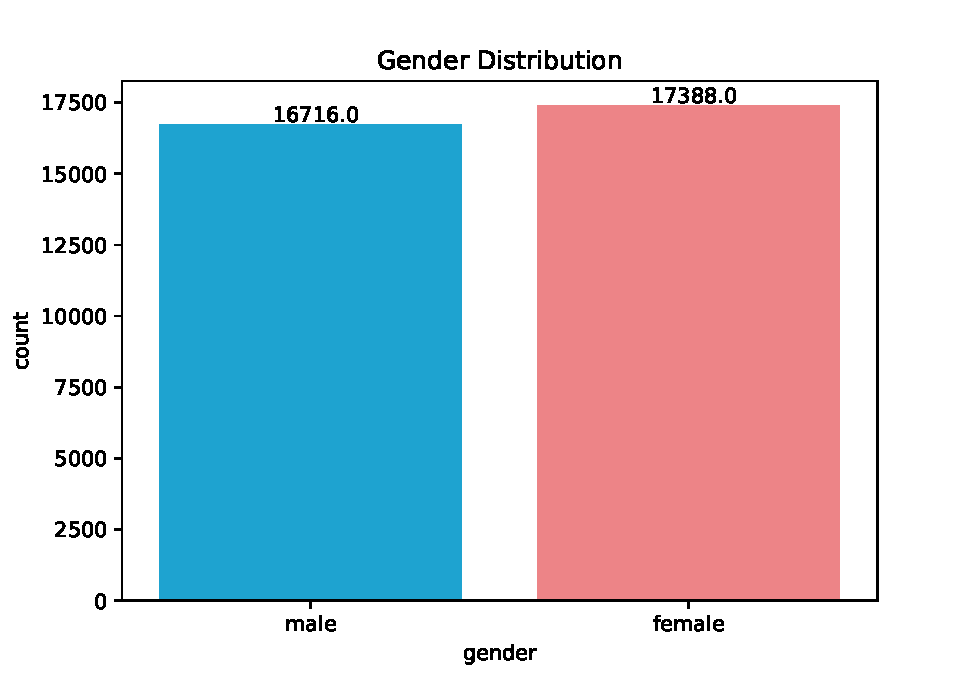
\includegraphics{term_paper_files/figure-latex/unnamed-chunk-6-1.pdf}

\hypertarget{education}{%
\subsubsection{\texorpdfstring{\emph{Education}}{Education}}\label{education}}

The \emph{Education} variable corresponds to the highest level of
education attained with `Primary', `Secondary' and `Tertiary' being the
three options. Here is the distribution of education by gender:

\begin{Shaded}
\begin{Highlighting}[]
\NormalTok{ebg }\OperatorTok{=}\NormalTok{ sns.countplot(x}\OperatorTok{=}\StringTok{"Education"}\NormalTok{, hue}\OperatorTok{=} \StringTok{"gender"}\NormalTok{, palette}\OperatorTok{=}\NormalTok{ gender\_palette, order}\OperatorTok{=}\NormalTok{ [}\StringTok{\textquotesingle{}Primary\textquotesingle{}}\NormalTok{, }\StringTok{\textquotesingle{}Secondary\textquotesingle{}}\NormalTok{, }\StringTok{\textquotesingle{}Tertiary\textquotesingle{}}\NormalTok{], data}\OperatorTok{=}\NormalTok{ df2)}
\ControlFlowTok{for}\NormalTok{ p }\KeywordTok{in}\NormalTok{ ebg.patches:}
\NormalTok{   ebg.annotate(}\StringTok{\textquotesingle{}}\SpecialCharTok{\{:.1f\}}\StringTok{\textquotesingle{}}\NormalTok{.}\BuiltInTok{format}\NormalTok{(p.get\_height()), (p.get\_x()}\OperatorTok{+}\FloatTok{.05}\NormalTok{, p.get\_height()}\OperatorTok{+}\DecValTok{100}\NormalTok{))}
\NormalTok{ebg.}\BuiltInTok{set}\NormalTok{(title}\OperatorTok{=} \StringTok{"Education Count by Gender"}\NormalTok{)}
\end{Highlighting}
\end{Shaded}

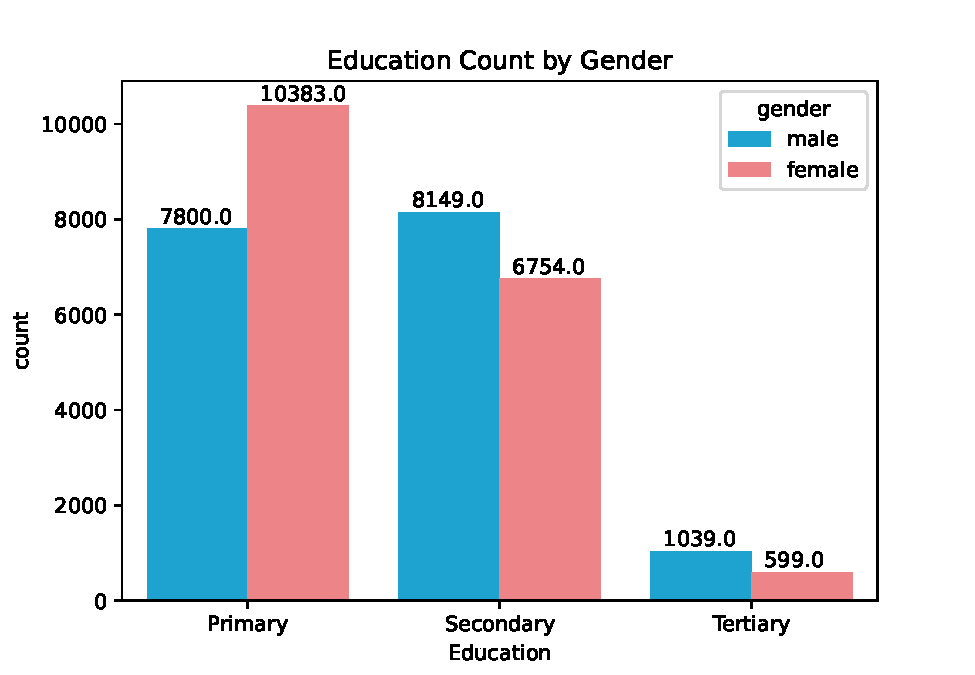
\includegraphics{term_paper_files/figure-latex/unnamed-chunk-7-3.pdf}

The bar plot above shows us that there are more women with primary
education, but more men with secondary or tertiary education. Overall,
we can see that there are more men with higher education than women.
About 1,000 more men have received a secondary education and there is
about double the amount of men with tertiary education compared to women
showing a clear disparity.

\hypertarget{economy}{%
\subsubsection{\texorpdfstring{\emph{economy}}{economy}}\label{economy}}

The final demographic variable of interest is the \emph{economy}
variable that separates respondents by which country they live in. There
are 35 different countries with exactly 1000 respondents from each.

\begin{Shaded}
\begin{Highlighting}[]
\CommentTok{\# Number of Observations per Country}
\NormalTok{plt.rcParams[}\StringTok{"figure.figsize"}\NormalTok{] }\OperatorTok{=}\NormalTok{ (}\DecValTok{10}\NormalTok{,}\DecValTok{7}\NormalTok{)}
\NormalTok{sns.countplot(y }\OperatorTok{=} \StringTok{\textquotesingle{}economy\textquotesingle{}}\NormalTok{, data }\OperatorTok{=}\NormalTok{ df2).}\BuiltInTok{set}\NormalTok{(title }\OperatorTok{=} \StringTok{"Distribution of Participants per Country"}\NormalTok{)}
\end{Highlighting}
\end{Shaded}

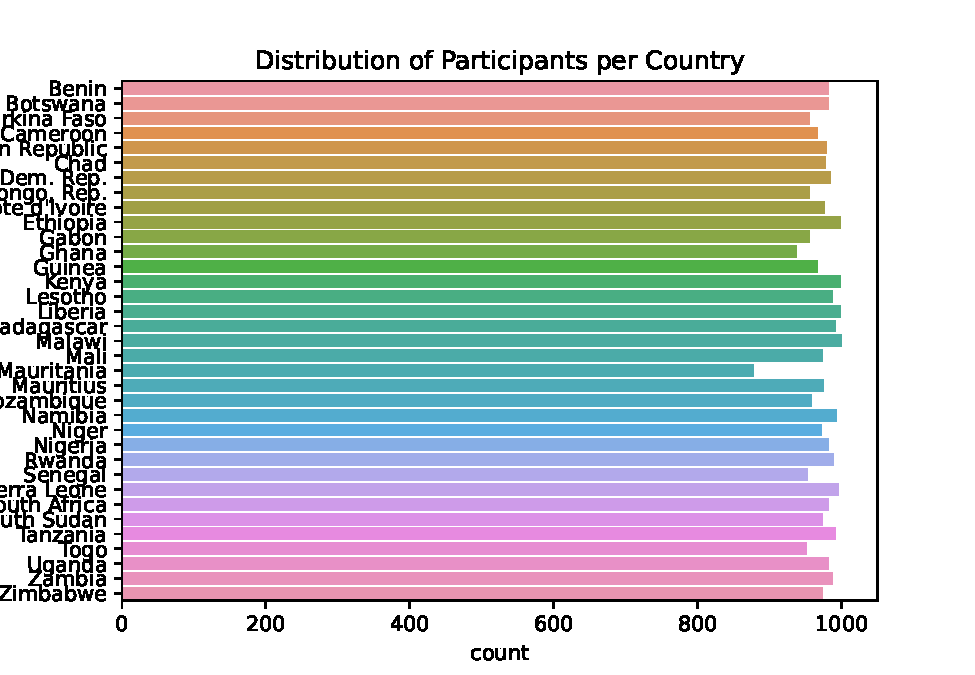
\includegraphics{term_paper_files/figure-latex/unnamed-chunk-8-5.pdf}

\hypertarget{financial}{%
\subsection{Financial}\label{financial}}

From the financial related variables, we were most interested in a few
specific financial variables that we thought would have an impact on
access to emergency funds.

\hypertarget{account_fin}{%
\subsubsection{\texorpdfstring{\emph{account\_fin}}{account\_fin}}\label{account_fin}}

The first variable being \emph{account\_fin} which distinguishes those
who have a financial account from those who don't:

\begin{Shaded}
\begin{Highlighting}[]
\CommentTok{\# barplot of number of people who have a bank account}
\NormalTok{g }\OperatorTok{=}\NormalTok{ sns.countplot(x }\OperatorTok{=} \StringTok{\textquotesingle{}account\_fin\textquotesingle{}}\NormalTok{, data }\OperatorTok{=}\NormalTok{ df2, palette }\OperatorTok{=}\NormalTok{ yes\_no\_pal)}
\ControlFlowTok{for}\NormalTok{ p }\KeywordTok{in}\NormalTok{ g.patches:}
\NormalTok{   g.annotate(}\StringTok{\textquotesingle{}}\SpecialCharTok{\{:.1f\}}\StringTok{\textquotesingle{}}\NormalTok{.}\BuiltInTok{format}\NormalTok{(p.get\_height()), (p.get\_x()}\OperatorTok{+} \FloatTok{.3}\NormalTok{, p.get\_height()}\OperatorTok{+}\DecValTok{100}\NormalTok{))}
\NormalTok{g.}\BuiltInTok{set}\NormalTok{(title }\OperatorTok{=} \StringTok{"Distribution of Has a Financial Account"}\NormalTok{, xlabel }\OperatorTok{=} \StringTok{\textquotesingle{}Has a financial account?\textquotesingle{}}\NormalTok{)}
\end{Highlighting}
\end{Shaded}

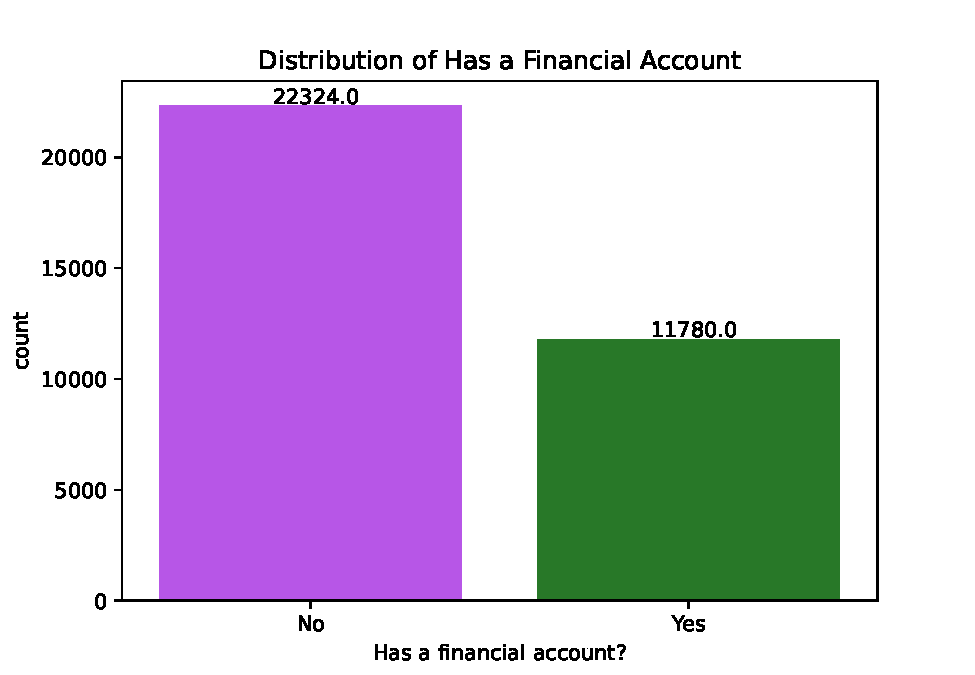
\includegraphics{term_paper_files/figure-latex/unnamed-chunk-9-7.pdf}

We can see that about two thirds of individuals do not have an account.
This is likely connected to the lack of access to emergency funds
displayed above given that if an individual does not have a financial
account, we would expect they are less likely to have a source of
emergency funds, as emergency funds are generally stored in an account.

\hypertarget{reason}{%
\subsubsection{\texorpdfstring{\emph{reason}}{reason}}\label{reason}}

Those who do not have a financial account were asked why in the
\emph{reason} variable, that provides a list of possible reasons for not
having a financial account:

\begin{Shaded}
\begin{Highlighting}[]
\CommentTok{\# reasons for no financial account}
\CommentTok{\# pivot data to long format}
\NormalTok{df\_long }\OperatorTok{=}\NormalTok{ df[[}\StringTok{\textquotesingle{}fin11a\textquotesingle{}}\NormalTok{, }\StringTok{"fin11b"}\NormalTok{, }\StringTok{"fin11c"}\NormalTok{, }\StringTok{"fin11d"}\NormalTok{, }\StringTok{"fin11e"}\NormalTok{, }\StringTok{"fin11f"}\NormalTok{, }\StringTok{"fin11g"}\NormalTok{, }\StringTok{"fin11h"}\NormalTok{]]}\OperatorTok{\textbackslash{}}
\NormalTok{.stack()}\OperatorTok{\textbackslash{}}
\NormalTok{.reset\_index()}
\NormalTok{df\_long.rename(columns }\OperatorTok{=}\NormalTok{ \{}\StringTok{\textquotesingle{}level\_1\textquotesingle{}}\NormalTok{:}\StringTok{\textquotesingle{}reason\textquotesingle{}}\NormalTok{, }\DecValTok{0}\NormalTok{:}\StringTok{\textquotesingle{}value\textquotesingle{}}\NormalTok{\}, inplace }\OperatorTok{=} \VariableTok{True}\NormalTok{)}
\NormalTok{df3 }\OperatorTok{=}\NormalTok{ df\_long.query(}\StringTok{\textquotesingle{}value == 1.0\textquotesingle{}}\NormalTok{) }\CommentTok{\# filter to only "yes" answers for each reason}
\CommentTok{\# recode reason values}
\NormalTok{df3.loc[df3[}\StringTok{\textquotesingle{}reason\textquotesingle{}}\NormalTok{] }\OperatorTok{==} \StringTok{\textquotesingle{}fin11a\textquotesingle{}}\NormalTok{, }\StringTok{"reason"}\NormalTok{] }\OperatorTok{=} \StringTok{\textquotesingle{}distance\textquotesingle{}}
\NormalTok{df3.loc[df3[}\StringTok{\textquotesingle{}reason\textquotesingle{}}\NormalTok{] }\OperatorTok{==} \StringTok{\textquotesingle{}fin11b\textquotesingle{}}\NormalTok{, }\StringTok{"reason"}\NormalTok{] }\OperatorTok{=} \StringTok{\textquotesingle{}expense\textquotesingle{}}
\NormalTok{df3.loc[df3[}\StringTok{\textquotesingle{}reason\textquotesingle{}}\NormalTok{] }\OperatorTok{==} \StringTok{\textquotesingle{}fin11c\textquotesingle{}}\NormalTok{, }\StringTok{"reason"}\NormalTok{] }\OperatorTok{=} \StringTok{\textquotesingle{}no\_documentation\textquotesingle{}}
\NormalTok{df3.loc[df3[}\StringTok{\textquotesingle{}reason\textquotesingle{}}\NormalTok{] }\OperatorTok{==} \StringTok{\textquotesingle{}fin11d\textquotesingle{}}\NormalTok{, }\StringTok{"reason"}\NormalTok{] }\OperatorTok{=} \StringTok{\textquotesingle{}lack\_trust\textquotesingle{}}
\NormalTok{df3.loc[df3[}\StringTok{\textquotesingle{}reason\textquotesingle{}}\NormalTok{] }\OperatorTok{==} \StringTok{\textquotesingle{}fin11e\textquotesingle{}}\NormalTok{, }\StringTok{"reason"}\NormalTok{] }\OperatorTok{=} \StringTok{\textquotesingle{}religious\textquotesingle{}}
\NormalTok{df3.loc[df3[}\StringTok{\textquotesingle{}reason\textquotesingle{}}\NormalTok{] }\OperatorTok{==} \StringTok{\textquotesingle{}fin11f\textquotesingle{}}\NormalTok{, }\StringTok{"reason"}\NormalTok{] }\OperatorTok{=} \StringTok{\textquotesingle{}lack\_money\textquotesingle{}}
\NormalTok{df3.loc[df3[}\StringTok{\textquotesingle{}reason\textquotesingle{}}\NormalTok{] }\OperatorTok{==} \StringTok{\textquotesingle{}fin11g\textquotesingle{}}\NormalTok{, }\StringTok{"reason"}\NormalTok{] }\OperatorTok{=} \StringTok{\textquotesingle{}family\_member\_has\textquotesingle{}}
\NormalTok{df3.loc[df3[}\StringTok{\textquotesingle{}reason\textquotesingle{}}\NormalTok{] }\OperatorTok{==} \StringTok{\textquotesingle{}fin11h\textquotesingle{}}\NormalTok{, }\StringTok{"reason"}\NormalTok{] }\OperatorTok{=} \StringTok{\textquotesingle{}no\_need\textquotesingle{}}
\NormalTok{df3.head()}

\CommentTok{\# aggregate counts by reason}
\end{Highlighting}
\end{Shaded}

\begin{verbatim}
##     level_0            reason  value
## 0     12138          distance    1.0
## 2     12138  no_documentation    1.0
## 11    12140        lack_trust    1.0
## 15    12140           no_need    1.0
## 18    12141  no_documentation    1.0
\end{verbatim}

\begin{Shaded}
\begin{Highlighting}[]
\NormalTok{reason\_counts }\OperatorTok{=}\NormalTok{ df3.groupby(}\StringTok{\textquotesingle{}reason\textquotesingle{}}\NormalTok{).agg(}\StringTok{\textquotesingle{}count\textquotesingle{}}\NormalTok{).reset\_index()}
\end{Highlighting}
\end{Shaded}

\begin{Shaded}
\begin{Highlighting}[]
\CommentTok{\# barplot of count by reason{-}{-} seaborn}
\NormalTok{reasons\_plot }\OperatorTok{=}\NormalTok{ sns.barplot(y }\OperatorTok{=} \StringTok{\textquotesingle{}reason\textquotesingle{}}\NormalTok{, x }\OperatorTok{=} \StringTok{\textquotesingle{}value\textquotesingle{}}\NormalTok{, data }\OperatorTok{=}\NormalTok{ reason\_counts, palette }\OperatorTok{=}\NormalTok{ [pink, pink, pink, pink, pink, pink, pink, pink], order }\OperatorTok{=}\NormalTok{ [}\StringTok{"lack\_money"}\NormalTok{,}\StringTok{"expense"}\NormalTok{,  }\StringTok{"no\_documentation"}\NormalTok{, }\StringTok{"distance"}\NormalTok{, }\StringTok{"lack\_trust"}\NormalTok{, }\StringTok{"no\_need"}\NormalTok{, }\StringTok{"family\_member\_has"}\NormalTok{, }\StringTok{"religious"}\NormalTok{]).}\BuiltInTok{set}\NormalTok{(title }\OperatorTok{=} \StringTok{"Reasons for No Financial Account"}\NormalTok{, xlabel }\OperatorTok{=} \StringTok{"count"}\NormalTok{)}
\end{Highlighting}
\end{Shaded}

\hypertarget{emp_in}{%
\subsubsection{\texorpdfstring{\emph{emp\_in}}{emp\_in}}\label{emp_in}}

Employment status was another financial variable of interest represented
by \emph{emp\_in}, which asks whether or not the participant is in the
workforce. It appears that about three-fourths of individuals are in the
workforce:

\begin{Shaded}
\begin{Highlighting}[]
\CommentTok{\# Distribution by in workforce}
\NormalTok{g }\OperatorTok{=}\NormalTok{ sns.countplot(x }\OperatorTok{=} \StringTok{\textquotesingle{}emp\_in\textquotesingle{}}\NormalTok{, data }\OperatorTok{=}\NormalTok{ df2, palette }\OperatorTok{=}\NormalTok{ yes\_no\_pal)}
\ControlFlowTok{for}\NormalTok{ p }\KeywordTok{in}\NormalTok{ g.patches:}
\NormalTok{   g.annotate(}\StringTok{\textquotesingle{}}\SpecialCharTok{\{:.1f\}}\StringTok{\textquotesingle{}}\NormalTok{.}\BuiltInTok{format}\NormalTok{(p.get\_height()), (p.get\_x()}\OperatorTok{+} \FloatTok{.3}\NormalTok{, p.get\_height()}\OperatorTok{+}\DecValTok{100}\NormalTok{))}
\NormalTok{g.}\BuiltInTok{set}\NormalTok{(title }\OperatorTok{=} \StringTok{"Distribution of Whether or not in Workforce"}\NormalTok{, xlabel }\OperatorTok{=} \StringTok{"In workforce?"}\NormalTok{)}
\end{Highlighting}
\end{Shaded}

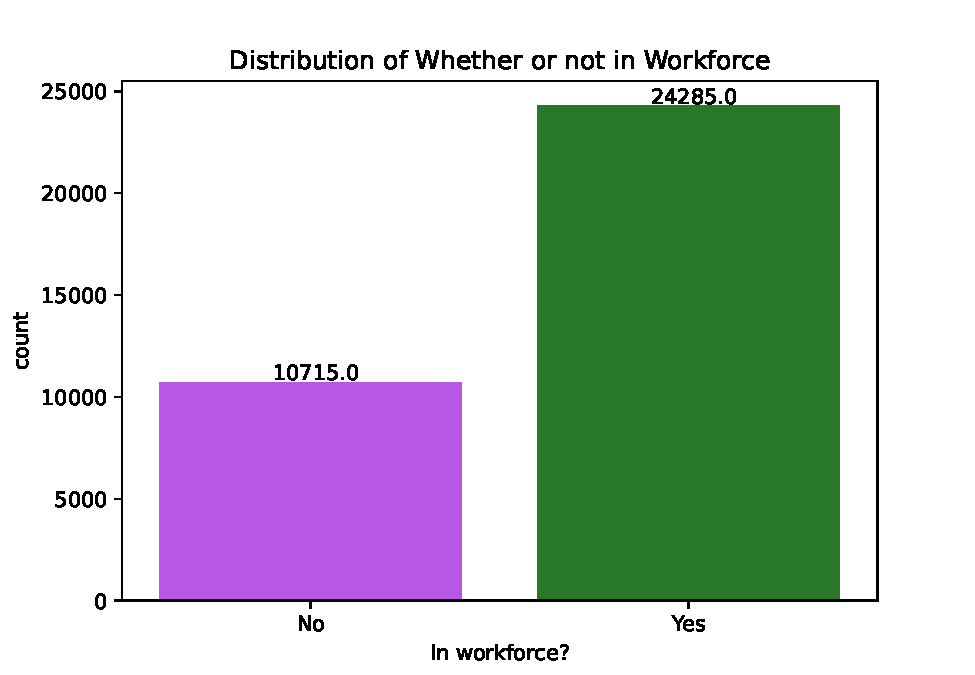
\includegraphics{term_paper_files/figure-latex/unnamed-chunk-12-9.pdf}

\hypertarget{inc_q}{%
\subsubsection{\texorpdfstring{\emph{inc\_q}}{inc\_q}}\label{inc_q}}

And lastly, we evaluated \emph{inc\_q}, which represents income
quantile. Income quantile is separated into 5 quantiles with 1 being the
poorest and 5 being the richest. The mean for all of the countries in
the dataset is 3.241. This means that all the countries average out to
be about middle class.

\begin{Shaded}
\begin{Highlighting}[]
\NormalTok{df\_inq }\OperatorTok{=}\NormalTok{ df[}\StringTok{\textquotesingle{}inc\_q\textquotesingle{}}\NormalTok{]}
\NormalTok{df[}\StringTok{"inc\_q"}\NormalTok{].mean()}
\CommentTok{\# fig = plt.figure()}
\CommentTok{\# ax1 = fig.add\_subplot(2,2,1) }
\CommentTok{\# sns.countplot(df\_inq, ax = ax1)}
\CommentTok{\# ax1.set\_xlabel("Income Quantile")}
\CommentTok{\# ax1.set\_xticklabels([\textquotesingle{}Poorest 20\%\textquotesingle{},\textquotesingle{}Second 20\%\textquotesingle{},\textquotesingle{}Middle 20\%\textquotesingle{},\textquotesingle{}Fourth 20\%\textquotesingle{},\textquotesingle{}Richest 20\%\textquotesingle{}])}
\CommentTok{\# ax1.title.set\_text(\textquotesingle{}Income Quantile  Distribution\textquotesingle{})}
\end{Highlighting}
\end{Shaded}

\begin{verbatim}
## 3.241085714285714
\end{verbatim}

The majority of the data set has individuals within the richest
quantile, Quantile 5.

\hypertarget{emergency-funds}{%
\subsection{Emergency Funds}\label{emergency-funds}}

To explore access to emergency funds in our dataset, we were interested
3 variables we thought could be related:

\hypertarget{has_access}{%
\subsubsection{\texorpdfstring{\emph{has\_access}}{has\_access}}\label{has_access}}

The variable \emph{has\_access} directly asks participants if they have
access to emergency funds:

\begin{Shaded}
\begin{Highlighting}[]
\CommentTok{\# barplot of access to emergency funds}
\NormalTok{g }\OperatorTok{=}\NormalTok{ sns.countplot(x }\OperatorTok{=} \StringTok{\textquotesingle{}has\_access\textquotesingle{}}\NormalTok{, data }\OperatorTok{=}\NormalTok{ df2, palette }\OperatorTok{=}\NormalTok{ yes\_no\_pal)}
\ControlFlowTok{for}\NormalTok{ p }\KeywordTok{in}\NormalTok{ g.patches:}
\NormalTok{   g.annotate(}\StringTok{\textquotesingle{}}\SpecialCharTok{\{:.1f\}}\StringTok{\textquotesingle{}}\NormalTok{.}\BuiltInTok{format}\NormalTok{(p.get\_height()), (p.get\_x()}\OperatorTok{+} \FloatTok{.25}\NormalTok{, p.get\_height()}\OperatorTok{+}\DecValTok{100}\NormalTok{))}
\NormalTok{g.}\BuiltInTok{set}\NormalTok{(title }\OperatorTok{=} \StringTok{"Distribution of Access to Emergency Funds"}\NormalTok{)}
\end{Highlighting}
\end{Shaded}

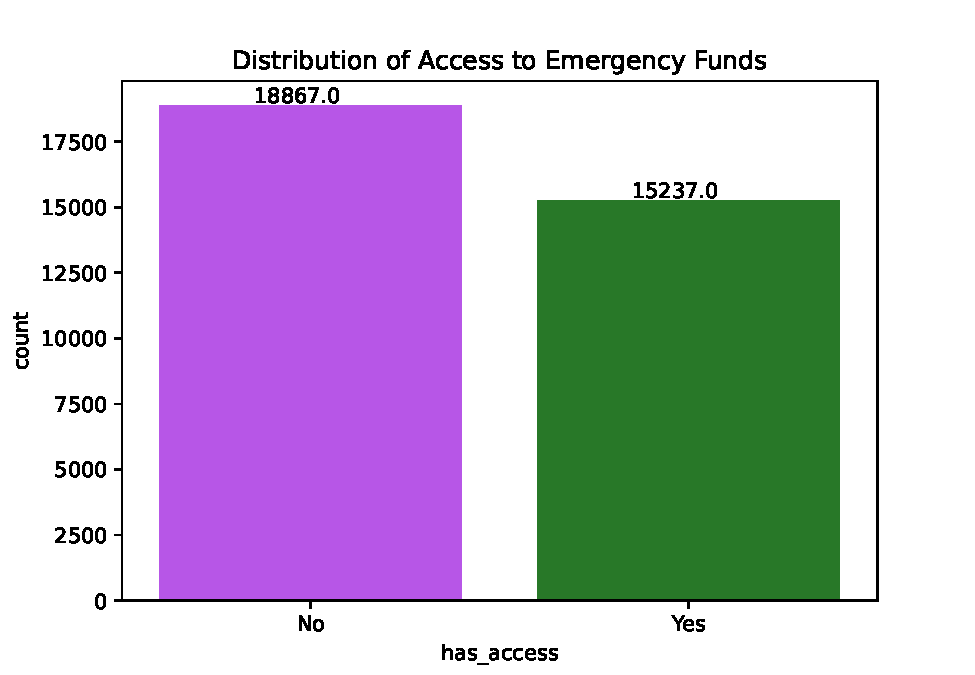
\includegraphics{term_paper_files/figure-latex/unnamed-chunk-14-11.pdf}

The barchart above displays the overall distribution of access to
emergency funds. We can see that over half of individuals represented in
the data do not have access.

\hypertarget{main_source_funds}{%
\subsubsection{\texorpdfstring{\emph{main\_source\_funds}}{main\_source\_funds}}\label{main_source_funds}}

We proceeded to explore the source of emergency funds using the
\emph{main\_source\_funds} variable, which provides a list of options
for where participants receive their main source of emergency funds:

\begin{Shaded}
\begin{Highlighting}[]
\CommentTok{\# barplot of main source of emergency funds}
\NormalTok{chart }\OperatorTok{=}\NormalTok{ sns.countplot(y }\OperatorTok{=} \StringTok{\textquotesingle{}main\_source\_funds\textquotesingle{}}\NormalTok{, }
\NormalTok{                      data }\OperatorTok{=}\NormalTok{ df2, }
\NormalTok{                      order }\OperatorTok{=}\NormalTok{ [}\StringTok{"Money from working"}\NormalTok{,}\StringTok{"Family, relatives, or friends"}\NormalTok{,}
                               \StringTok{"Savings"}\NormalTok{, }\StringTok{"Selling assets"}\NormalTok{,}
                               \StringTok{"Borrowing from a bank/employer/private lender"}\NormalTok{, }\StringTok{"(Some other source)"}\NormalTok{]).}\BuiltInTok{set}\NormalTok{(}
\NormalTok{                      title }\OperatorTok{=} \StringTok{"Distribution of the Main Source of Emergency Funds"}\NormalTok{)}
\end{Highlighting}
\end{Shaded}

The barchart above displays the overall distribution of the main source
of emergency funds. Most of the individuals with access to emergency
funds receive their funding from work, their family and friends, or
their savings.

\hypertarget{recieve-wage-payments}{%
\subsubsection{\texorpdfstring{\emph{Recieve Wage
Payments}}{Recieve Wage Payments}}\label{recieve-wage-payments}}

Diving further into the ``Money from Working'' category, we can see that
only 8196 individuals receive wage payments from the \emph{Receive Wage
Payments} variable. This analysis suggests that receiving wage payments
may be a key factor in determining access to emergency funds.

\begin{Shaded}
\begin{Highlighting}[]
\CommentTok{\# barplot of recieved wage payments}
\NormalTok{chart }\OperatorTok{=}\NormalTok{ sns.countplot(x }\OperatorTok{=} \StringTok{\textquotesingle{}Receive Wage Payments\textquotesingle{}}\NormalTok{,data }\OperatorTok{=}\NormalTok{ df2, order }\OperatorTok{=}\NormalTok{ [}\StringTok{"No"}\NormalTok{, }\StringTok{"Yes"}\NormalTok{], palette }\OperatorTok{=}\NormalTok{ yes\_no\_pal)}
\ControlFlowTok{for}\NormalTok{ p }\KeywordTok{in}\NormalTok{ chart.patches:}
\NormalTok{   chart.annotate(}\StringTok{\textquotesingle{}}\SpecialCharTok{\{:.1f\}}\StringTok{\textquotesingle{}}\NormalTok{.}\BuiltInTok{format}\NormalTok{(p.get\_height()), (p.get\_x()}\OperatorTok{+} \FloatTok{.25}\NormalTok{, p.get\_height()}\OperatorTok{+}\DecValTok{100}\NormalTok{))}
\NormalTok{chart.}\BuiltInTok{set}\NormalTok{(title }\OperatorTok{=} \StringTok{"Distribution of Received Wage Payments"}\NormalTok{)}
\end{Highlighting}
\end{Shaded}

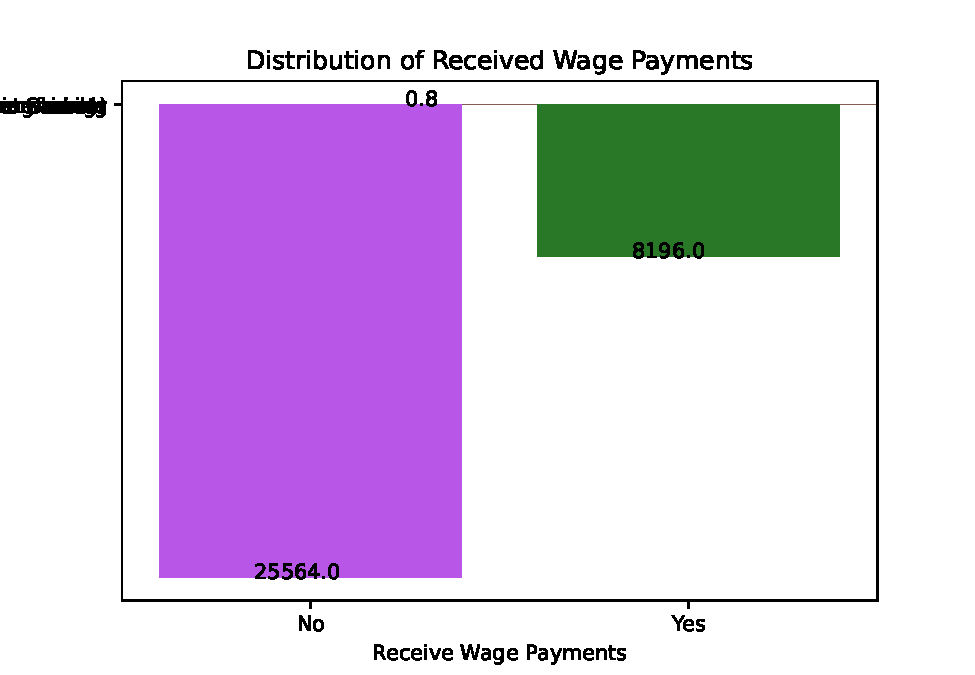
\includegraphics{term_paper_files/figure-latex/unnamed-chunk-16-13.pdf}

\hypertarget{gender-economy-and-education-in-relation-to-emergency-funds}{%
\subsubsection{\texorpdfstring{\emph{gender}, \emph{economy} and
\emph{Education} in relation to Emergency
Funds}{gender, economy and Education in relation to Emergency Funds}}\label{gender-economy-and-education-in-relation-to-emergency-funds}}

Finally, we sought to find if there were disparities in access to
emergency funds by \emph{gender}, \emph{economy}, and \emph{Education}.

\begin{Shaded}
\begin{Highlighting}[]
\NormalTok{df\_gender }\OperatorTok{=}\NormalTok{ df2[[}\StringTok{\textquotesingle{}gender\textquotesingle{}}\NormalTok{, }\StringTok{\textquotesingle{}economy\textquotesingle{}}\NormalTok{]].query(}\StringTok{"gender == \textquotesingle{}female\textquotesingle{}"}\NormalTok{).groupby(}\StringTok{\textquotesingle{}economy\textquotesingle{}}\NormalTok{).count()}
\NormalTok{df\_gender }\OperatorTok{=}\NormalTok{ df\_gender.assign(male }\OperatorTok{=} \KeywordTok{lambda}\NormalTok{ df\_gender: }\DecValTok{1000} \OperatorTok{{-}}\NormalTok{ df\_gender[}\StringTok{\textquotesingle{}gender\textquotesingle{}}\NormalTok{]).rename(columns }\OperatorTok{=}\NormalTok{ \{}\StringTok{\textquotesingle{}gender\textquotesingle{}}\NormalTok{: }\StringTok{\textquotesingle{}female\textquotesingle{}}\NormalTok{\})}
 
\CommentTok{\#Percent of females}
\NormalTok{df\_gender }\OperatorTok{=}\NormalTok{ df\_gender.assign(Female }\OperatorTok{=} \KeywordTok{lambda}\NormalTok{ df\_gender: (df\_gender[}\StringTok{\textquotesingle{}female\textquotesingle{}}\NormalTok{])}\OperatorTok{/}\DecValTok{10}\NormalTok{)}
 
\CommentTok{\#Percent of males}
\NormalTok{df\_gender }\OperatorTok{=}\NormalTok{ df\_gender.assign(Male }\OperatorTok{=} \KeywordTok{lambda}\NormalTok{ df\_gender: }\DecValTok{100} \OperatorTok{{-}}\NormalTok{ df\_gender[}\StringTok{\textquotesingle{}Female\textquotesingle{}}\NormalTok{])}
 
\NormalTok{df\_gender }\OperatorTok{=}\NormalTok{ df\_gender[[}\StringTok{\textquotesingle{}Male\textquotesingle{}}\NormalTok{, }\StringTok{\textquotesingle{}Female\textquotesingle{}}\NormalTok{]]}
\NormalTok{df\_gender[}\StringTok{\textquotesingle{}economy\textquotesingle{}}\NormalTok{] }\OperatorTok{=}\NormalTok{ df2.economy.unique()}
\NormalTok{df\_gender }\OperatorTok{=}\NormalTok{ df\_gender.sort\_values(}\StringTok{\textquotesingle{}Male\textquotesingle{}}\NormalTok{)}
 
\CommentTok{\# Counting by Access to Emergency Funds by gender}
\NormalTok{f\_access }\OperatorTok{=}\NormalTok{ df2[[}\StringTok{\textquotesingle{}has\_access\textquotesingle{}}\NormalTok{, }\StringTok{\textquotesingle{}economy\textquotesingle{}}\NormalTok{, }\StringTok{\textquotesingle{}gender\textquotesingle{}}\NormalTok{]].query(}\StringTok{"has\_access == \textquotesingle{}Yes\textquotesingle{} \& gender == \textquotesingle{}female\textquotesingle{}"}\NormalTok{).groupby(}\StringTok{\textquotesingle{}economy\textquotesingle{}}\NormalTok{).count()}
\NormalTok{m\_access }\OperatorTok{=}\NormalTok{ df2[[}\StringTok{\textquotesingle{}has\_access\textquotesingle{}}\NormalTok{, }\StringTok{\textquotesingle{}economy\textquotesingle{}}\NormalTok{, }\StringTok{\textquotesingle{}gender\textquotesingle{}}\NormalTok{]].query(}\StringTok{"has\_access == \textquotesingle{}Yes\textquotesingle{}\& gender != \textquotesingle{}female\textquotesingle{}"}\NormalTok{).groupby(}\StringTok{\textquotesingle{}economy\textquotesingle{}}\NormalTok{).count()}

\CommentTok{\# Defining acccess vs no access by country columms}
\NormalTok{f\_count }\OperatorTok{=}\NormalTok{ f\_access[}\StringTok{\textquotesingle{}has\_access\textquotesingle{}}\NormalTok{]}
\NormalTok{m\_count }\OperatorTok{=}\NormalTok{ m\_access[}\StringTok{\textquotesingle{}has\_access\textquotesingle{}}\NormalTok{]}
 
\CommentTok{\# Merging columns}
\NormalTok{df3 }\OperatorTok{=}\NormalTok{ pd.merge(f\_count, m\_count, how}\OperatorTok{=}\StringTok{\textquotesingle{}inner\textquotesingle{}}\NormalTok{, on }\OperatorTok{=} \StringTok{\textquotesingle{}economy\textquotesingle{}}\NormalTok{)}
\NormalTok{df3 }\OperatorTok{=}\NormalTok{ df3.assign(total }\OperatorTok{=} \KeywordTok{lambda}\NormalTok{ df3: df3[}\StringTok{\textquotesingle{}has\_access\_x\textquotesingle{}}\NormalTok{]}\OperatorTok{+}\NormalTok{df3[}\StringTok{\textquotesingle{}has\_access\_y\textquotesingle{}}\NormalTok{])}
 
\CommentTok{\#Percent of females with access}
\NormalTok{df3 }\OperatorTok{=}\NormalTok{ df3.assign(f\_percent\_access }\OperatorTok{=} \KeywordTok{lambda}\NormalTok{ df3: (df3[}\StringTok{\textquotesingle{}has\_access\_x\textquotesingle{}}\NormalTok{]}\OperatorTok{/}\NormalTok{df3[}\StringTok{"total"}\NormalTok{])}\OperatorTok{*}\DecValTok{100}\NormalTok{)}
 
\CommentTok{\#Percent of males with access}
\NormalTok{df3 }\OperatorTok{=}\NormalTok{ df3.assign(m\_percent\_access }\OperatorTok{=} \DecValTok{100} \OperatorTok{{-}}\NormalTok{ df3[}\StringTok{\textquotesingle{}f\_percent\_access\textquotesingle{}}\NormalTok{])}
 
\NormalTok{df3[}\StringTok{\textquotesingle{}economy\textquotesingle{}}\NormalTok{] }\OperatorTok{=}\NormalTok{ df2.economy.unique()}
\NormalTok{df3 }\OperatorTok{=}\NormalTok{ df3[[}\StringTok{\textquotesingle{}m\_percent\_access\textquotesingle{}}\NormalTok{, }\StringTok{\textquotesingle{}f\_percent\_access\textquotesingle{}}\NormalTok{,   }\StringTok{\textquotesingle{}economy\textquotesingle{}}\NormalTok{]]}
\NormalTok{df3 }\OperatorTok{=}\NormalTok{ df3.sort\_values(}\StringTok{\textquotesingle{}m\_percent\_access\textquotesingle{}}\NormalTok{)}
\NormalTok{df3 }\OperatorTok{=}\NormalTok{ df3.rename(columns }\OperatorTok{=}\NormalTok{ \{}\StringTok{\textquotesingle{}m\_percent\_access\textquotesingle{}}\NormalTok{:}\StringTok{\textquotesingle{}Males With Acesss\textquotesingle{}}\NormalTok{, }\StringTok{\textquotesingle{}f\_percent\_access\textquotesingle{}}\NormalTok{: }\StringTok{\textquotesingle{}Females With Access\textquotesingle{}}\NormalTok{\})}
\end{Highlighting}
\end{Shaded}

\begin{Shaded}
\begin{Highlighting}[]
\CommentTok{\# create new figure}
\NormalTok{fig }\OperatorTok{=}\NormalTok{ plt.figure()}
\CommentTok{\#add sub plot}
\end{Highlighting}
\end{Shaded}

\begin{verbatim}
## <string>:1: MatplotlibDeprecationWarning: The resize_event function was deprecated in Matplotlib 3.6 and will be removed two minor releases later. Use callbacks.process('resize_event', ResizeEvent(...)) instead.
\end{verbatim}

\begin{Shaded}
\begin{Highlighting}[]
\NormalTok{ax1 }\OperatorTok{=}\NormalTok{ fig.add\_subplot(}\DecValTok{1}\NormalTok{,}\DecValTok{2}\NormalTok{,}\DecValTok{1}\NormalTok{)}
\CommentTok{\# fig 1}
\NormalTok{df\_gender.set\_index(}\StringTok{\textquotesingle{}economy\textquotesingle{}}\NormalTok{).plot(kind}\OperatorTok{=}\StringTok{\textquotesingle{}barh\textquotesingle{}}\NormalTok{, stacked}\OperatorTok{=}\VariableTok{True}\NormalTok{, color}\OperatorTok{=}\NormalTok{[}\StringTok{\textquotesingle{}steelblue\textquotesingle{}}\NormalTok{, }\StringTok{\textquotesingle{}pink\textquotesingle{}}\NormalTok{], title }\OperatorTok{=} \StringTok{"Percent of Participants by Country \& Gender"}\NormalTok{, ax }\OperatorTok{=}\NormalTok{ ax1).axvline(x }\OperatorTok{=} \DecValTok{50}\NormalTok{, color }\OperatorTok{=} \StringTok{"red"}\NormalTok{, linestyle }\OperatorTok{=} \StringTok{"dashed"}\NormalTok{)}
\CommentTok{\#add sub plot}
\NormalTok{ax2 }\OperatorTok{=}\NormalTok{ fig.add\_subplot(}\DecValTok{1}\NormalTok{,}\DecValTok{2}\NormalTok{,}\DecValTok{2}\NormalTok{)}
\CommentTok{\# fig 2}
\NormalTok{fig2 }\OperatorTok{=}\NormalTok{ df3.set\_index(}\StringTok{\textquotesingle{}economy\textquotesingle{}}\NormalTok{).plot(kind}\OperatorTok{=}\StringTok{\textquotesingle{}barh\textquotesingle{}}\NormalTok{, stacked}\OperatorTok{=}\VariableTok{True}\NormalTok{, color}\OperatorTok{=}\NormalTok{[}\StringTok{\textquotesingle{}steelblue\textquotesingle{}}\NormalTok{, }\StringTok{\textquotesingle{}pink\textquotesingle{}}\NormalTok{], title }\OperatorTok{=} \StringTok{"Percent of Participants with Access to Emergency Funds by Country \& Gender"}\NormalTok{, ax }\OperatorTok{=}\NormalTok{ ax2).axvline(x }\OperatorTok{=} \DecValTok{50}\NormalTok{, color }\OperatorTok{=} \StringTok{"red"}\NormalTok{, linestyle }\OperatorTok{=} \StringTok{"dashed"}\NormalTok{)}
\CommentTok{\# set fig size}
\NormalTok{fig.set\_size\_inches(}\DecValTok{29}\NormalTok{, }\DecValTok{14}\NormalTok{)}
\end{Highlighting}
\end{Shaded}

In the side-by-side barplots above, we can see that although only about
50\% of the countries have a higher percentage of men represented in the
questionnaire (left bar plot), in 75\% of the countries more men have
access to emergency funds than women (right bar plot).

\begin{Shaded}
\begin{Highlighting}[]
\CommentTok{\# Counting by Access to Emergency Funds by country}
\NormalTok{access }\OperatorTok{=}\NormalTok{ df2[[}\StringTok{\textquotesingle{}has\_access\textquotesingle{}}\NormalTok{, }\StringTok{\textquotesingle{}economy\textquotesingle{}}\NormalTok{]].query(}\StringTok{"has\_access == \textquotesingle{}Yes\textquotesingle{}"}\NormalTok{).groupby(}\StringTok{\textquotesingle{}economy\textquotesingle{}}\NormalTok{).count()}
\NormalTok{no\_access }\OperatorTok{=}\NormalTok{ df2[[}\StringTok{\textquotesingle{}has\_access\textquotesingle{}}\NormalTok{, }\StringTok{\textquotesingle{}economy\textquotesingle{}}\NormalTok{]].query(}\StringTok{"has\_access == \textquotesingle{}No\textquotesingle{}"}\NormalTok{).groupby(}\StringTok{\textquotesingle{}economy\textquotesingle{}}\NormalTok{).count()}
 
\CommentTok{\# Defining acccess vs no access by country columms}
\NormalTok{a\_count }\OperatorTok{=}\NormalTok{ access[}\StringTok{\textquotesingle{}has\_access\textquotesingle{}}\NormalTok{]}
\NormalTok{no\_a\_count }\OperatorTok{=}\NormalTok{ no\_access[}\StringTok{\textquotesingle{}has\_access\textquotesingle{}}\NormalTok{]}
 
\CommentTok{\# Merging columns}
\NormalTok{df3 }\OperatorTok{=}\NormalTok{ pd.merge(a\_count, no\_a\_count, how}\OperatorTok{=}\StringTok{\textquotesingle{}inner\textquotesingle{}}\NormalTok{, on }\OperatorTok{=} \StringTok{\textquotesingle{}economy\textquotesingle{}}\NormalTok{)}\CommentTok{\#.assign(total = lambda df3: df3[\textquotesingle{}has\_access\_x\textquotesingle{}]+df3[\textquotesingle{}has\_access\_y\textquotesingle{}])}
\CommentTok{\#df3 = df3.assign(percent\_access = lambda df3: (df3[\textquotesingle{}has\_access\_x\textquotesingle{}]/df3["total"])*100)}
 
\NormalTok{df3[}\StringTok{\textquotesingle{}economy\textquotesingle{}}\NormalTok{] }\OperatorTok{=}\NormalTok{ df2.economy.unique()}
\NormalTok{df3 }\OperatorTok{=}\NormalTok{ df3.sort\_values(}\StringTok{\textquotesingle{}has\_access\_x\textquotesingle{}}\NormalTok{)}


\NormalTok{educ\_perc }\OperatorTok{=}\NormalTok{ (df2.groupby([}\StringTok{\textquotesingle{}Education\textquotesingle{}}\NormalTok{])[}\StringTok{\textquotesingle{}has\_access\textquotesingle{}}\NormalTok{]}
\NormalTok{                     .value\_counts(normalize}\OperatorTok{=}\VariableTok{True}\NormalTok{)}
\NormalTok{                     .rename(}\StringTok{\textquotesingle{}percentage\textquotesingle{}}\NormalTok{)}
\NormalTok{                     .mul(}\DecValTok{100}\NormalTok{)}
\NormalTok{                     .reset\_index()}
\NormalTok{                     )}
\end{Highlighting}
\end{Shaded}

\begin{Shaded}
\begin{Highlighting}[]
\NormalTok{educ\_access }\OperatorTok{=}\NormalTok{ sns.barplot(x }\OperatorTok{=} \StringTok{"Education"}\NormalTok{, y }\OperatorTok{=} \StringTok{"percentage"}\NormalTok{, order}\OperatorTok{=}\NormalTok{ [}\StringTok{\textquotesingle{}Primary\textquotesingle{}}\NormalTok{, }\StringTok{\textquotesingle{}Secondary\textquotesingle{}}\NormalTok{, }\StringTok{\textquotesingle{}Tertiary\textquotesingle{}}\NormalTok{], hue}\OperatorTok{=}\StringTok{"has\_access"}\NormalTok{, palette}\OperatorTok{=}\NormalTok{ yes\_no\_pal, hue\_order}\OperatorTok{=}\NormalTok{ [}\StringTok{\textquotesingle{}No\textquotesingle{}}\NormalTok{, }\StringTok{\textquotesingle{}Yes\textquotesingle{}}\NormalTok{], data }\OperatorTok{=}\NormalTok{ educ\_perc)}
\ControlFlowTok{for}\NormalTok{ p }\KeywordTok{in}\NormalTok{ educ\_access.patches:}
\NormalTok{   educ\_access.annotate(}\StringTok{\textquotesingle{}}\SpecialCharTok{\{:.1f\}}\StringTok{\textquotesingle{}}\NormalTok{.}\BuiltInTok{format}\NormalTok{(p.get\_height()), (p.get\_x()}\OperatorTok{+}\FloatTok{.12}\NormalTok{, p.get\_height()}\OperatorTok{+}\FloatTok{.5}\NormalTok{))}
\NormalTok{educ\_access.}\BuiltInTok{set}\NormalTok{(title }\OperatorTok{=} \StringTok{"Access to Emergency Funds by Education Level"}\NormalTok{, xlabel }\OperatorTok{=} \StringTok{\textquotesingle{}Education Level\textquotesingle{}}\NormalTok{)}
\end{Highlighting}
\end{Shaded}

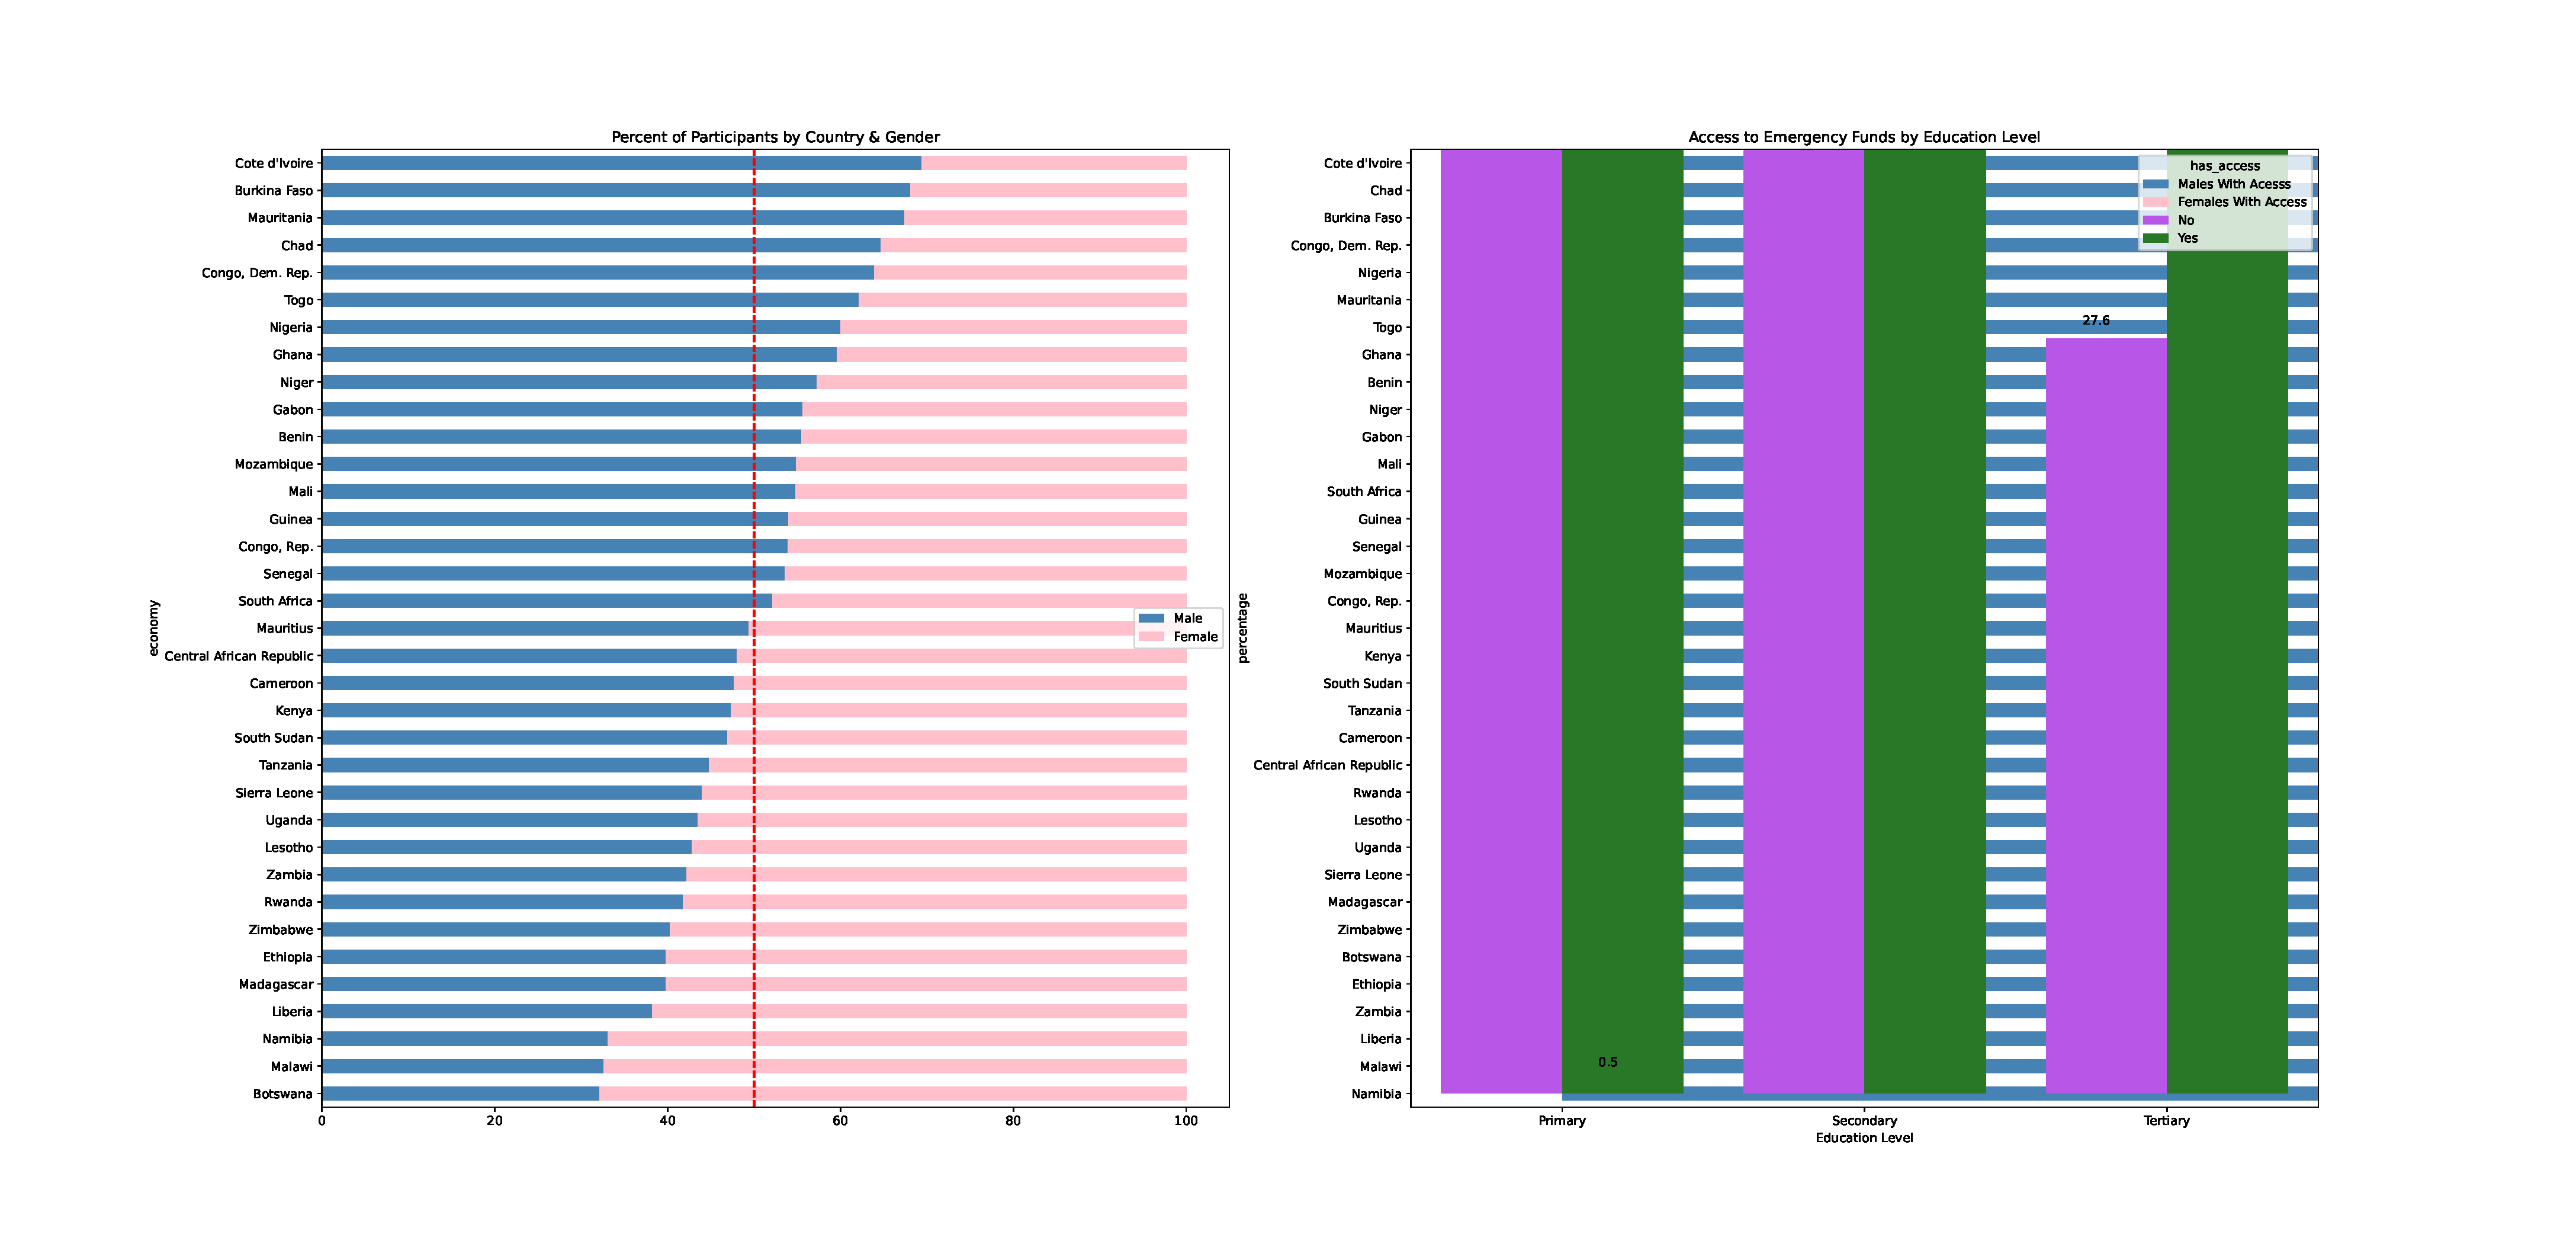
\includegraphics{term_paper_files/figure-latex/unnamed-chunk-20-15.pdf}

Additionally, in the barplot above we can see the distribution of funds
based on an individual's highest education level. 63\% of people with
only a primary education do not have access to emergency funds compared
to 37\% of people who do. These numbers are more evenly distributed for
those with secondary education, with about 49\% of people not having
access to emergency funds, while 51\% of people do have access. Finally,
for those with a tertiary level of education we can see that about 72\%
of people have access to emergency funds while only 28\% of that group
does not have access. Overall, we can make the assumption that people
with a higher level of education are more likely to have access to
emergency funds.

\hypertarget{materials-and-methods}{%
\section{Materials and Methods}\label{materials-and-methods}}

Materials and Methods \citep{knight_automated_2020} should be described
with sufficient details to allow others to replicate and build on
published results. Please note that publication of your manuscript
implicates that you must make all materials, data, computer code, and
protocols associated with the publication available to readers. Please
disclose at the submission stage any restrictions on the availability of
materials or information. New methods and protocols should be described
in detail while well-established methods can be briefly described and
appropriately cited.\citep{kypraiou_what_2021}

Research manuscripts reporting large datasets that are deposited in a
publicly available database should specify where the data have been
deposited and provide the relevant accession numbers. If the accession
numbers have not yet been obtained at the time of submission, please
state that they will be provided during review. They must be provided
prior to publication.\citep{gebru_datasheets_2021}

Interventionary studies involving animals or humans, and other studies
require ethical approval must list the authority that provided approval
and the corresponding ethical approval code.

\hypertarget{results}{%
\section{Results}\label{results}}

This section may be divided by subheadings. It should provide a concise
and precise description of the experimental results, their
interpretation as well as the experimental conclusions that can be
drawn.\citep{barocas_fairness_nodate}

\hypertarget{subsection-heading-here}{%
\subsection{Subsection Heading Here}\label{subsection-heading-here}}

Subsection text here.

\hypertarget{subsubsection-heading-here}{%
\subsubsection{Subsubsection Heading
Here}\label{subsubsection-heading-here}}

Bulleted lists look like this:

\begin{itemize}
\tightlist
\item
  First bullet
\item
  Second bullet
\item
  Third bullet
\end{itemize}

Numbered lists can be added as follows:

\begin{enumerate}
\def\labelenumi{\arabic{enumi}.}
\tightlist
\item
  First item
\item
  Second item
\item
  Third item
\end{enumerate}

The text continues here.

All figures and tables should be cited in the main text as Figure 1,
Table 1, etc.

\begin{figure}[H]
\centering

\includegraphics[width=3 cm]{logo-mdpi}
\caption{This is a figure, Schemes follow the same formatting. If there are multiple panels, they should be listed as: (\textbf{a}) Description of what is contained in the first panel. (\textbf{b}) Description of what is contained in the second panel. Figures should be placed in the main text near to the first time they are cited. A caption on a single line should be centered.}
\end{figure}

\begin{table}[H]
\caption{This is a table caption. Tables should be placed in the main text near to the first time they are cited.}
\centering
%% \tablesize{} %% You can specify the fontsize here, e.g.  \tablesize{\footnotesize}. If commented out \small will be used.
\begin{tabular}{ccc}
\toprule
\textbf{Title 1}    & \textbf{Title 2}  & \textbf{Title 3}\\
\midrule
entry 1     & data          & data\\
entry 2     & data          & data\\
\bottomrule
\end{tabular}
\end{table}

This is an example of an equation:

\begin{equation}
\mathbb{S}
\end{equation}

Example of a theorem:

\begin{Theorem}
Example text of a theorem.
\end{Theorem}

The text continues here. Proofs must be formatted as follows:

Example of a proof:

\begin{proof}[Proof of Theorem 1]
Text of the proof. Note that the phrase `of Theorem 1' is optional if it is clear which theorem is being referred to.
\end{proof}

The text continues here.

\hypertarget{discussion}{%
\section{Discussion}\label{discussion}}

Authors should discuss the results and how they can be interpreted in
perspective of previous studies and of the working hypotheses. The
findings and their implications should be discussed in the broadest
context possible. Future research directions may also be highlighted.

\hypertarget{conclusion}{%
\section{Conclusion}\label{conclusion}}

This section is not mandatory, but can be added to the manuscript if the
discussion is unusually long or complex.

\hypertarget{patents}{%
\section{Patents}\label{patents}}

This section is not mandatory, but may be added if there are patents
resulting from the work reported in this manuscript.

% %%%%%%%%%%%%%%%%%%%%%%%%%%%%%%%%%%%%%%%%%%
% %% optional
% \supplementary{The following are available online at www.mdpi.com/link, Figure S1: title, Table S1: title, Video S1: title.}
%
% % Only for the journal Methods and Protocols:
% % If you wish to submit a video article, please do so with any other supplementary material.
% % \supplementary{The following are available at www.mdpi.com/link: Figure S1: title, Table S1: title, Video S1: title. A supporting video article is available at doi: link.}

\vspace{6pt}

%%%%%%%%%%%%%%%%%%%%%%%%%%%%%%%%%%%%%%%%%%
\acknowledgments{All sources of funding of the study should be
disclosed. Please clearly indicate grants that you have received in
support of your research work. Clearly state if you received funds for
covering the costs to publish in open access.}

%%%%%%%%%%%%%%%%%%%%%%%%%%%%%%%%%%%%%%%%%%
\authorcontributions{For research articles with several authors, a short
paragraph specifying their individual contributions must be provided.
The following statements should be used ``X.X. and Y.Y. conceive and
designed the experiments; X.X. performed the experiments; X.X. and Y.Y.
analyzed the data; W.W. contributed reagents/materials/analysis tools;
Y.Y. wrote the paper.'\,' Authorship must be limited to those who have
contributed substantially to the work reported.}

%%%%%%%%%%%%%%%%%%%%%%%%%%%%%%%%%%%%%%%%%%
\conflictsofinterest{Declare conflicts of interest or state `The authors
declare no conflict of interest.' Authors must identify and declare any
personal circumstances or interest that may be perceived as
inappropriately influencing the representation or interpretation of
reported research results. Any role of the funding sponsors in the
design of the study; in the collection, analyses or interpretation of
data in the writing of the manuscript, or in the decision to publish the
results must be declared in this section. If there is no role, please
state `The founding sponsors had no role in the design of the study; in
the collection, analyses, or interpretation of data; in the writing of
the manuscript, an in the decision to publish the results'.}

%%%%%%%%%%%%%%%%%%%%%%%%%%%%%%%%%%%%%%%%%%
%% optional
\abbreviations{The following abbreviations are used in this manuscript:\\

\noindent
\begin{tabular}{@{}ll}
MDPI & Multidisciplinary Digital Publishing Institute \\
DOAJ & Directory of open access journals \\
TLA & Three letter acronym \\
LD & linear dichroism \\
\end{tabular}}

\input{"appendix.tex"}

%%%%%%%%%%%%%%%%%%%%%%%%%%%%%%%%%%%%%%%%%%
% Citations and References in Supplementary files are permitted provided that they also appear in the reference list here.

%=====================================
% References, variant A: internal bibliography
%=====================================
%\reftitle{References}
%\begin{thebibliography}{999}
% Reference 1
%\bibitem[Author1(year)]{ref-journal}
%Author1, T. The title of the cited article. {\em Journal Abbreviation} {\bf 2008}, {\em 10}, 142--149.
% Reference 2
%\bibitem[Author2(year)]{ref-book}
%Author2, L. The title of the cited contribution. In {\em The Book Title}; Editor1, F., Editor2, A., Eds.; Publishing House: City, Country, 2007; pp. 32--58.
%\end{thebibliography}

% The following MDPI journals use author-date citation: Arts, Econometrics, Economies, Genealogy, Humanities, IJFS, JRFM, Laws, Religions, Risks, Social Sciences. For those journals, please follow the formatting guidelines on http://www.mdpi.com/authors/references
% To cite two works by the same author: \citeauthor{ref-journal-1a} (\citeyear{ref-journal-1a}, \citeyear{ref-journal-1b}). This produces: Whittaker (1967, 1975)
% To cite two works by the same author with specific pages: \citeauthor{ref-journal-3a} (\citeyear{ref-journal-3a}, p. 328; \citeyear{ref-journal-3b}, p.475). This produces: Wong (1999, p. 328; 2000, p. 475)

%=====================================
% References, variant B: external bibliography
%=====================================
\reftitle{References}
\externalbibliography{yes}
\bibliography{mybibfile.bib}

%%%%%%%%%%%%%%%%%%%%%%%%%%%%%%%%%%%%%%%%%%
%% optional
\sampleavailability{Samples of the compounds \ldots\ldots{} are
available from the authors.}

%% for journal Sci
%\reviewreports{\\
%Reviewer 1 comments and authors’ response\\
%Reviewer 2 comments and authors’ response\\
%Reviewer 3 comments and authors’ response
%}

%%%%%%%%%%%%%%%%%%%%%%%%%%%%%%%%%%%%%%%%%%


\end{document}
